\chapter{Experiment 1}
\label{ch:4}

\section{Introduction}

Experiment 1 of the current study investigates the accentedness of various phonetic patterns in non- native (L2) English speech. The current study considers the most common native (L1) English productions observed in one hundred L1 speakers of American English as the L1 target productions (e.g., [æsk] for “\textit{ask}”). L2 speech productions that differ from the L1 target productions were considered mismatches. The mismatch stimuli, therefore, represent patterns in L2 speech that do not match the most common L1 productions.

Eleven types of consonant mismatches, 5 types of vowel mismatches and 2 types of syllable structure mismatches were assembled to enable a detailed comparison between different types of speech patterns in L2 speech. The stimuli were chosen based on their phonetic transcriptions (IPA transcriptions), which were vetted by at least 3 professional transcribers and were further examined by acoustic analysis conducted by the current study, as described in Chapter \ref{ch:3}.

L1 American English raters were recruited from the Amazon Mechanical Turk (MTurk) platform to provide accentedness judgments on the stimuli. The results provide direct comparisons between the accentendess of different types of consonant, vowel and syllable structural patterns in L2 speech.


\section{Stimuli}

Stimuli for the current study were selected based on their respective phonetic transcriptions, which were verified by acoustic analysis conducted as part of the current study (Chapters \ref{ch:3}). An example of the four types of stimuli were introduced in Chapter \ref{ch:3} and are re-listed here in Table 4.1, where the “Contexts” column specifies the five phonological contexts. There are 20 stimuli for each of the 5 contexts, yielding 100 stimuli in total.

% Table generated by Excel2LaTeX from sheet 'stimuli'
\begin{table}[!h]
  \figSpace
  \centering
  \caption{Types of Stimuli}
\label{table:tos2}
    \begin{tabular}{p{5.2em}llll}
    \toprule
    Contexts & \multicolumn{1}{p{5.2em}}{Match} & \multicolumn{1}{p{5em}}{Consonant\quad Mismatch} & \multicolumn{1}{p{5em}}{Vowel\quad Mismatch} & \multicolumn{1}{p{5em}}{Syllable\quad Mismatch} \\
    \midrule
    \textit{please call} &[pʰliz kʰɑl]&[\textbf{p}liz kʰɑl]&[pʰliz kʰ\textbf{o}l]&[pʰ\textbf{ə}liz kʰɑl] \\
     \textit{ask her} &[æsk (h)əɹ] &[æsk hə\textbf{r}]&[\textbf{ɑ}sk həɹ]&[æs\underline{ } həɹ]\\
     \textit{six spoons} &[sɪks spunz]&[sɪks spun\textbf{ʃ}]&[s\textbf{i}ks spunz]&[sɪks \textbf{ə}spunz] \\
     \textit{five thick} &[faɪv θɪk]&[faɪv \textbf{t}ɪk] &[f\textbf{a}v θɪk]&[faɪv\textbf{ə} θɪk]\\
     \textit{small plastic} &[smɑl pʰlæstɪk]&[smɑ\textbf{ɭ} pʰlæstɪk]&[smɑl pʰlæst\textbf{i}k]&[smɑl pʰlæs\underline{ }ɪk] \\
    \bottomrule
    \end{tabular}%
      \figSpace
\end{table}%

IPA transcriptions of the match stimuli are the same as IPA transcriptions of their L1 target productions (e.g.  [θɪk] for “\textit{thick}”), meaning that the IPA transcriptions of the match stimuli match IPA transcriptions of their L1 target productions. L2 speech samples that do not match their L1 target productions were termed the mismatch stimuli. The mismatch stimuli were further divided into three groups based on three types of mismatches, namely, stimuli with consonant mismatches (e.g., [tɪk] for “\textit{thick}”), stimuli with vowel mismatches (e.g., [θik] for “\textit{thick}”), and stimuli with syllable structure mismatches (e.g., [faɪvə] for “\textit{five}”). Experiment 1 therefore investigates four types of stimuli (i.e., the match stimuli and the three types of mismatch stimuli).


\section{Procedure}
 
Experiment 1 recruited L1 listeners of American English to provide accentedness ratings of the 100 stimuli. Participants (i.e., raters) heard each of the 100 audio stimuli and were then asked to judge the degree of the foreign accent exhibited in the stimulus on a 9-point Likert-like scale (Figure \ref{fig:exp1}). Following the practice of similar studies (e.g., McCullough, 2013), only the endpoints of the scale were marked. 

The raters heard the 100 audio stimuli without knowing the intended meaning of the stimuli. A rating of one means the stimulus has no foreign accent at all. A rating of nine means the stimulus has a very strong foreign accent.

The interface of the experiment provided a button and a 9-point rating scale. Raters were instructed to wear headphones or earbuds to listen to the stimuli\footnote{Since the experiment was conducted online, we cannot ensure that all the raters wore headphones or earbuds during the experiment. This could be a potential methodological limitation. Readers could consult \citet{Woods_2017} for a psychophysical test that helps to determine whether online experiment participants are wearing headphones.}. A stimulus was played once the rater hit the button, after which the rating scale would appear. Raters provided their accentedness judgment by choosing a number from one to nine on the rating scale, and then moved on to the next trial. There was no time limit for each trial. The maximum time allowed for completing the entire experiment was 30 minutes. Figure \ref{fig:exp1} illustrates the interface of the experiment.

\begin{figure}[!h]
  \figSpace
    \centering
	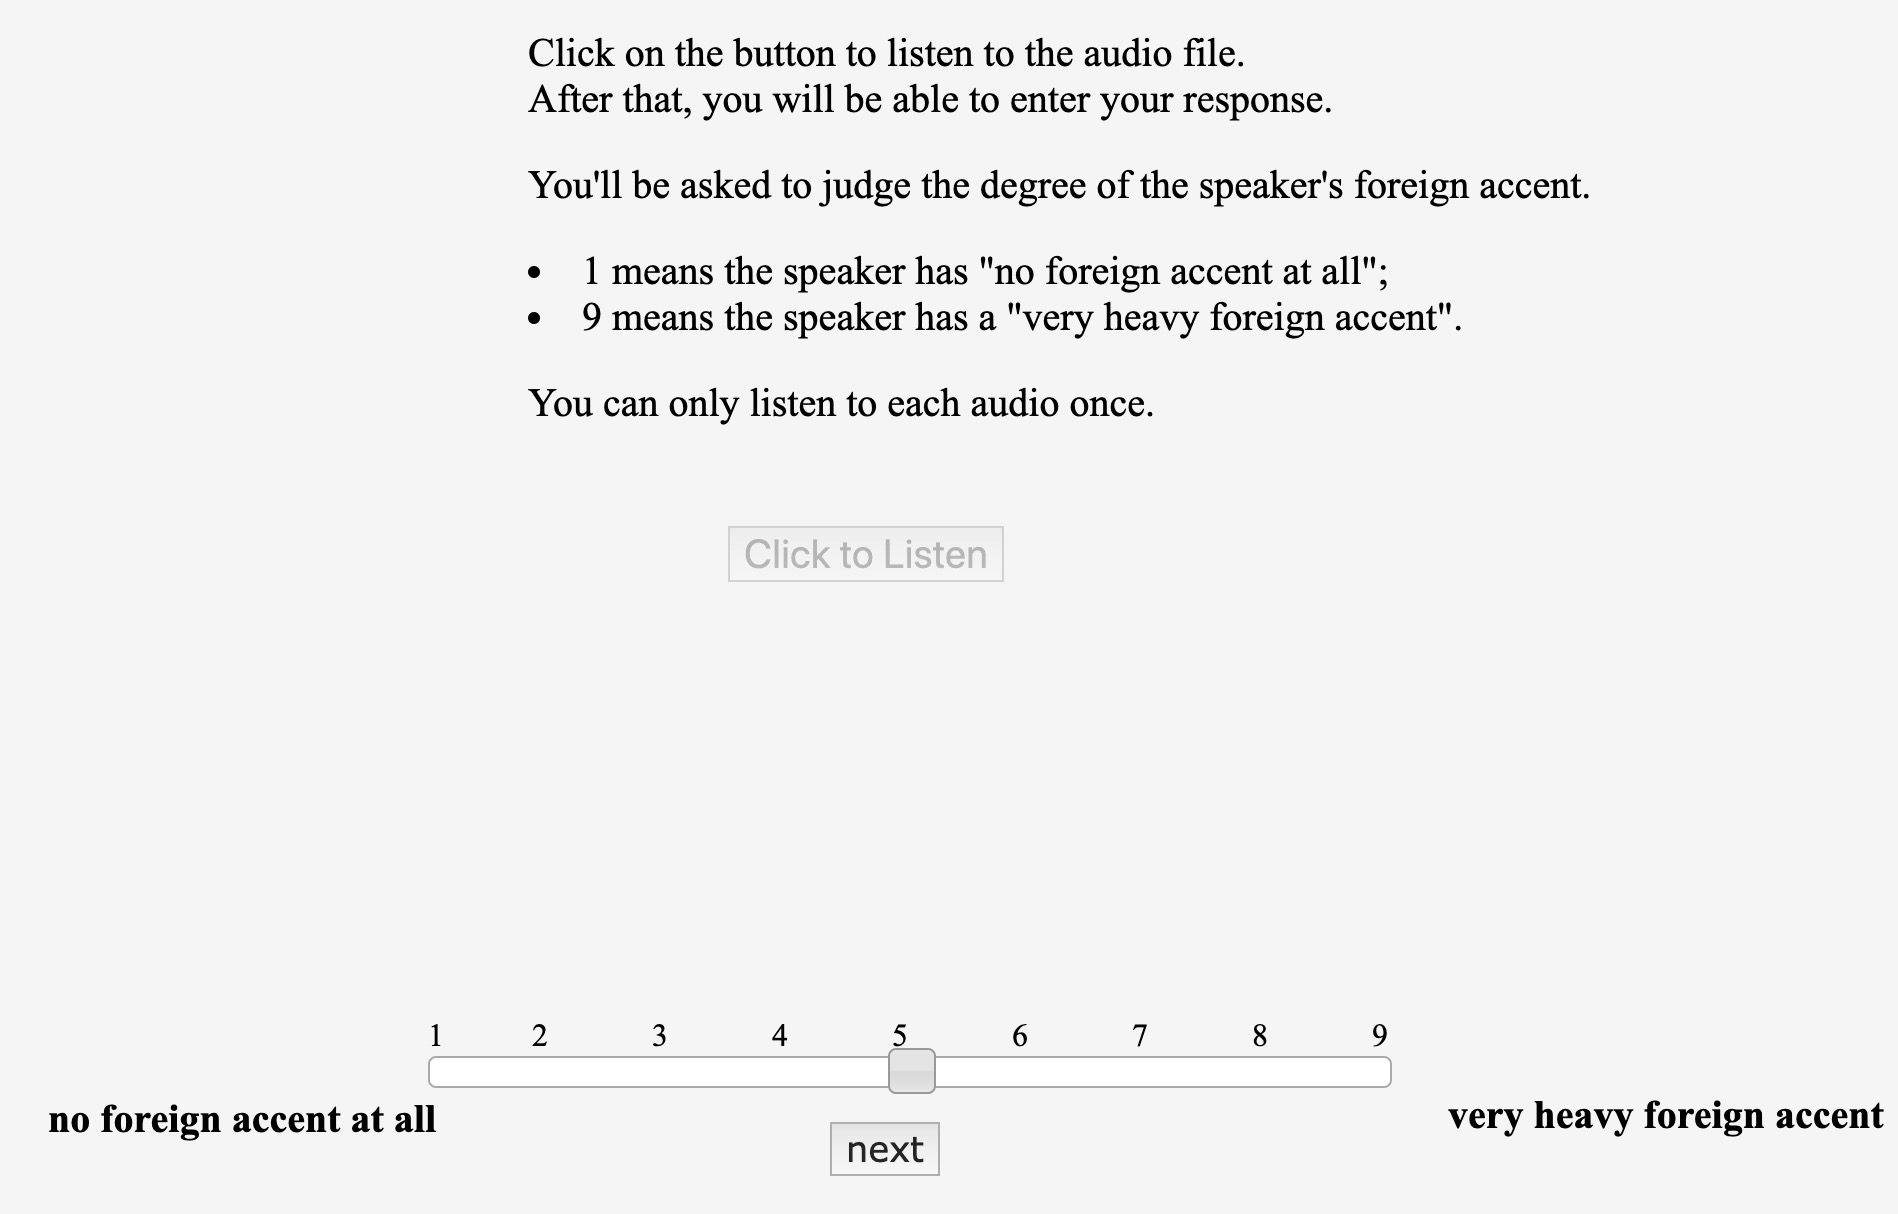
\includegraphics[width=0.75\textwidth]{figures/exp1.jpg}
    \caption{Interface of Experiment 1}
    \label{fig:exp1}
  \figSpace
\end{figure}

To reduce the order-effect, a block randomization technique was implemented. The 100 stimuli were divided into five blocks, each of which contained one token per type per context, yielding 20 stimuli per block (five contexts × four types). The order of blocks and the stimuli in each block were randomized for each participant via JavaScript using the Fisher-Yates Shuffle algorithm \citep{Fisher_1963}. 

 Raters of Experiment 1 were not required to identify or locate the specific type of mismatch in each stimulus, because the mismatch had already been determined by the vetted transcriptions.

There were 100 trials in total. At the end of the experiment, the raters were asked to take a demo- graphics survey, which collected information on the raters’ age, gender, L1/L2 status, occupation, current residence and birthplace. Raters on average spent 12.3 minutes (SD=3.2 minutes) on the experiment. Raters were compensated \$0.50 upon completion of the experiment. The experiment was programmed with HTML, CSS and JavaScript.

Previous studies often provide a training session to familiarize participants with the range of accents in the experiment \citep{Major_1986, Munro_1999}. However, the conundrum is that there is no way to obtain the full range of accents without testing the raters first. Experimenters could subjectively select a few representative stimuli for the training session, but ex- perimenters’ own biases could be introduced in the process. Experiment 1 therefore opted to omit the training session. The Result section of this chapter discusses how the absence of training affects raters’ accentedness judgments.


\section{Raters}
\label{rater:1}
Participants (i.e., raters) were 110 adult L1 American English speakers recruited via Amazon Me- chanical Turk (MTurk), a web-application that allows researchers to conduct survey-based experi- ments. Previous literature has shown that results of behavioral experiments conducted on MTurk are comparable to results of similar experiments conducted in lab settings \citep{Enochson_2015, Sprouse_2010}. \citet{Difallah_2018} recently showed that there are about 2,000 participants active on MTurk at any given time. 51\% of them are female, 49\% of them are male. About 75\% of the participants are from the United States. Indian participants represent 16\% of the population. The rest are from Canada, Great Britain, the Philippines and Germany.

Since Experiment 1 aims to investigate accentedness judgments of American English listeners, the experiment was made accessible only to people with a U.S. IP address. To increase the reliability of responses, the experiment required participants to have an approval rating of at least 95\%. That is, at least 95\% of each participant’s previous work on MTurk has met the requirements of the people who assigned the work.  All of the participants reported their birth location and residence as being in the United States. All of them reported that that they are L1 speakers of English. We therefore assumed that the participants are L1 speakers of American English. Two of the participants reported having speech or hearing related disorders. Responses from these two participants were thus removed, yielding 108 participants in total, among which 61 were female, 45 were male, and two did not report their gender. The age of the 108 participants ranged from 20 to 66. The mean age was 33.50 (SD=12.51) (See rater demographics in Appendix B).

\section{Control for Prosody}
\label{ch4:prosody}

The current study focuses specifically on segmental and syllable structure information. However, prosodic information has often been shown to affect foreign accent perception (e.g., \citealp{Magen_1998, Munro_1995}). It is therefore important for the current study to control for prosodic information of the selected stimuli. The following section first reviews the methods used by previous studies and then describes the method implemented by the current study.

 Two types of methods were often used in previous research to account for prosodic information. One method, usually termed \textit{prosody cloning} or \textit{prosody transplantation}, involves the superimposing of prosody of one utterance onto another \citep{Mareuil_2006, Yoon_2007}. At least two utterances are required with this method. Usually, highly controlled read speech samples are used, so that the two utterances contain exactly the same number of segments. The duration, fundamental frequency (F0), or intensity of segments in one utterance (the “donor”) can be automatically superimposed on the other utterance (the “recipient”) via the PSOLA algorithm \citep{Moulines_1990}. In this way, the recipient sample may have similar or even identical prosodic characteristics as the donor. 

The drawback of this method is that the number of segments in the donor and the recipient should be the same, which might cause problems for imposing L1 prosody on L2 speech with epenthesis or segment deletion. Moreover, acoustic manipulations of prosody will probably alter the acoustic characteristics in segmental dimensions, which might artificially increase or decrease accentedness of the original speech. Therefore, it might not be ideal to implement this method in studies that investigate segmental characteristics of foreign accent. 

An alternative method measures the prosodic differences without acoustic manipulation. This method implements the Dynamic Time Warping (DTW) alignment algorithm to account for the prosodic difference between two utterances \citep{Adami_2003, Rilliard_2011, Sharpe_2015}. DTW is a non-linear algorithm that looks for the dissimilarity between two temporal sequences of data and calculates the costs to align one with the other.  It generates a DTW score that represents the dissimilarity between two sets of data. The greater the DTW score, the more dissimilar the two sets of data are. 

The advantages of the DTW method are that (1) it does not involve any acoustic manipulation of the original speech files; (2) it does not require that the two utterances compared contain the same number of segments, which make it suitable for comparing L1 and L2 speech samples that differ in syllable structure; and (3) the calculation not only compares F0 and/or intensity values at different time points, but also takes into account the durational difference between two utterances, where larger differences will lead to a greater DTW score. In other words, the DTW score might, to some degree, represent the global prosodic differences of two utterances. The DTW method could thus be more suitable for the current study. 

In the current study, the DTW algorithm took F0 values of L1 speech samples as the reference and F0 values of an L2 speech sample as the input. The algorithm generated DTW scores, which represent the intonational and durational dissimilarities between the L1 and L2 speech samples.  L1 productions were first analyzed to find L1 F0 contours. Male and female speech samples were separately processed. For each gender, speech samples were grouped by the five contexts. F0 contours of the speech samples were extracted using the PRAAT auto-correlation algorithm \citep{Boersma_2015}. The contours were then divided into 300 equally spaced time points for every second (i.e., 3.33 ms per point), from which an F0 value was extracted. Following \citet{Morrill_2015}, gaps in the contour were interpolated from the points on either side of the gap. Artifacts were removed by smoothing with a bandwidth of 5 Hz. F0 values were then converted to semitones relative to 100 Hz. Pitch range for female speech samples was set between 100 Hz and 500 Hz. Pitch range for male speech samples was set between 75 Hz and 300 Hz. To allow for cross-speaker comparison, the semitones were then normalized for each speaker. 

F0 values of the 100 L2 stimuli were similarly extracted and normalized. The DTW algorithm was then implemented in R with the \textit{dtw} package \citep{Giorgino_2009} to calculate the degree of prosodic dissimilarity between L1 and L2 speech samples. For every L2 stimulus, 25 DTW scores were generated to represent the warping cost between the L2 stimulus and each of its corresponding 25 L1 speech samples. The mean DTW scores for each L2 stimulus were then calculated to account for prosodic information of the stimulus. The mean DTW scores for all of the 100 L2 stimuli were recorded for further statistical analysis. 

\section{Results}
\subsection{Experiment 1 Hypotheses}
Based on previous research on speech perception and lexical identification, Experiment 1 hypothesizes that stimuli with consonant mismatches are perceptually more foreign-accented than stimuli with vowel mismatches, because consonants are more susceptible to categorical perception than vowels and are more important in lexical identification. Based on previous empirical findings on L2 speech perception, Experiment 1 predicts that segment epenthesis is perceptually more foreign-accented than segment deletion, because segment deletion is sometimes allowed in L1 speech, while segment epenthesis rarely occurs. Experiment 1 also predicts that stimuli with mismatches should be generally more foreign-accented than stimuli without mismatches (i.e., the match stimuli).

\subsection{Segmental and Structural Mismatches}

The mean ratings across all four stimulus types (each stimulus was rated on a scale from 1 to 9) was 4.81 (SD=2.21). The larger the number, the more foreign-accented a stimulus was judged. As expected, raters assigned higher ratings for stimuli with mismatches (M=5.10, SD=2.15) than for stimuli without mismatches (M=3.94, SD=2.16). Ratings of stimuli with consonant mismatches (M=5.66, SD=2.04) were on average higher than ratings of stimuli with syllable structural mismatches (M=4.96, SD=2.17), which were on average higher than ratings of stimuli with vowel mismatches (M=4.69, SD=2.13). Figure \ref{fig:bar1} demonstrates the mean ratings of the four types of stimuli, where the error bars represent the 95\% confidence intervals. 

\begin{figure}[!h]
  \figSpace
\centering
%bar1 for Exp1
\begin{tikzpicture}
  \begin{axis}[
  ylabel={Mean Ratings},
width=9.2cm,
   height = 7cm,
    ytick distance=1,
        nodes near coords,
      major x tick style = transparent,
    ybar=3*\pgflinewidth,
      bar width=30pt,
      ymajorgrids = true,
      symbolic x coords={Match,Vowel,Syllable,Consonant},
      xtick ={Match,Vowel, Syllable, Consonant},
      scaled y ticks = false,
        legend style={at={(1.2,0.55)},
  anchor=north},
  legend cell align=left,
      enlarge x limits=0.20,
      ymin=0,
       every axis plot/.append style={
          ybar,
          bar shift=0pt,
          fill
        }
    ]
\addplot [fill=mycolor4,error bars/.cd, y dir=both, y explicit,error bar style=black] 
  coordinates {
          (Match, 3.94) += (0,0.08) -= (0,0.08)};
\addplot [fill=mycolor3,error bars/.cd, y dir=both, y explicit,error bar style=black] 
  coordinates {
          (Vowel, 4.69) += (0,0.08) -= (0,0.08)};
\addplot [fill=mycolor2,error bars/.cd, y dir=both, y explicit,error bar style=black] 
  coordinates {
          (Syllable, 4.96) += (0,0.08) -= (0,0.08)};
 \addplot [fill=mycolor1,error bars/.cd, y dir=both, y explicit,error bar style=black] 
  coordinates {
          (Consonant, 5.66) += (0,0.08) -= (0,0.08)};
 \end{axis}
\end{tikzpicture}



\caption{Mean Ratings by Type of Stimuli on the Scale from 1 to 9}
\label{fig:bar1}
\figSpace
\end{figure}

Linear mixed-effects models were employed with the \textit{lme4} package in R \citep{Bates_2014} to investigate the possible influence of the segmental and syllable mismatches on foreign accent ratings. In the full model, the dependent variable was the ratings. Type of stimuli (consonant mismatch vs. vowel mismatches vs. syllable mismatch vs. match) was Helmert contrast-coded to examine whether the four types of stimuli affect accentedness rating differently. Three stimuli contrasts were created. The first contrast compared consonant mismatch with syllable mismatch; the second contrast compared vowel mismatch with consonant and syllable mismatch; and the third contrast compared the three types of mismatch stimuli with the match stimuli. To investigate accentedness ratings across the 100 trials, trial numbers were also included as a fixed effect. To control for prosody, the mean DTW score of each stimulus was included as a fixed effect. The interactions among the three stimuli contrasts, the trial number and the DTW scores were also included as fixed effects. Raters were included as a random effect with the “type of stimuli” as its random slope. Stimuli were included as another random effect.

The effects of fixed effect factors were investigated by comparing models using the likelihood ratio test. The full model was as described above. The likelihood ratio test is a test of the goodness-of-fit between two models. It produces a chi-square and a p-value to indicate whether one model fits a particular set of data significantly better than the other model. To investigate the contribution of a particular fixed effect to model fit, the fixed effect needs to be removed from the full model to construct a new model. The new model, therefore, differs from the full model only by the exclusion of one single parameter (i.e., the particular fixed effect factor). If the full model indeed fits the dataset significantly better than the new model, then one could conclude that the exclusion of the specific fixed effect factor significantly changed the model fit, which implies that the fixed effect factor in question is statistically significant. 

To investigate the effect of DTW scores, the fixed effect factor DTW cores was removed from the full model to construct a new model.  The new model was compared to the full model using the likelihood ratio test. The result showed that the full model did not fit the dataset significantly better than the new model (χ2 = 2.87, p =.09), indicating that the contribution of DTW scores to model fit was not significant. The same method was applied to the investigation on other fixed effects. The results show that none of the interactions involving DTW scores achieved significant contribution to model fit, suggesting that the intonation of the stimuli might not be a major factor affecting accentedness ratings. 

The contrast between consonant and syllable mismatches significantly contributed to model fit (χ2 = 6.35, p < .05), showing that stimuli with consonant mismatches were rated as being more accented than stimuli with syllable mismatches. The second contrast, which compares vowel mismatches with consonant and syllable mismatches, contributed significantly to model fit (χ2 = 6.95, p < .01), showing that stimuli with consonant mismatches and syllable mismatches were rated as being more accented than stimuli with vowel mismatches. The third contrast, which compares the match stimuli with the three types of mismatch stimuli, also contributed significantly to model fit (χ2 = 13.32, p < .001), showing that stimuli with segmental and structural mismatches were perceived as being more accented than the match stimuli. 

These results suggest that all of the three types of mismatches contributed to the perception of foreign accent. However, stimuli with consonant mismatches were perceived as being more accented than the other two. Among the three types of mismatches, stimuli with vowel mismatches were perceived to be the least accented. The DTW scores, which represent prosodic differences between L1 and L2 productions, positively correlated with accentedness ratings. The contribution of the DTW scores to model fit was only marginally significant, suggesting that prosodic influence might not be a major factor that affected accentedness ratings. 

\subsection{Ratings across Time}

The comparison of models also revealed a significant effect of trial numbers on accentedness ratings (β=0.03, χ2 = 46.80, p < .001), suggesting that ratings were not consistent across the 100 trials. That is, the same stimuli might receive different ratings depending on when it occurred during the experiment. More specifically, the later a stimulus occurred in the experiment, the more accented the stimulus was rated. The interaction between trial number and the third contrast contributed significantly to model fit (β=0.04, χ2 = 9.87, p < .01), showing that stimuli with segmental and structural mismatches became more accented than the match stimuli as the experiment progressed. Figure \ref{fig:trial1} demonstrates the accentedness rating across time, where the ribbons represent the 95\% confidence intervals. The accentedness ratings increased as the experiment progressed. 

\begin{figure}[h!]
  \figSpace
    \centering
% Created by tikzDevice version 0.12.3 on 2019-11-24 19:33:25
% !TEX encoding = UTF-8 Unicode
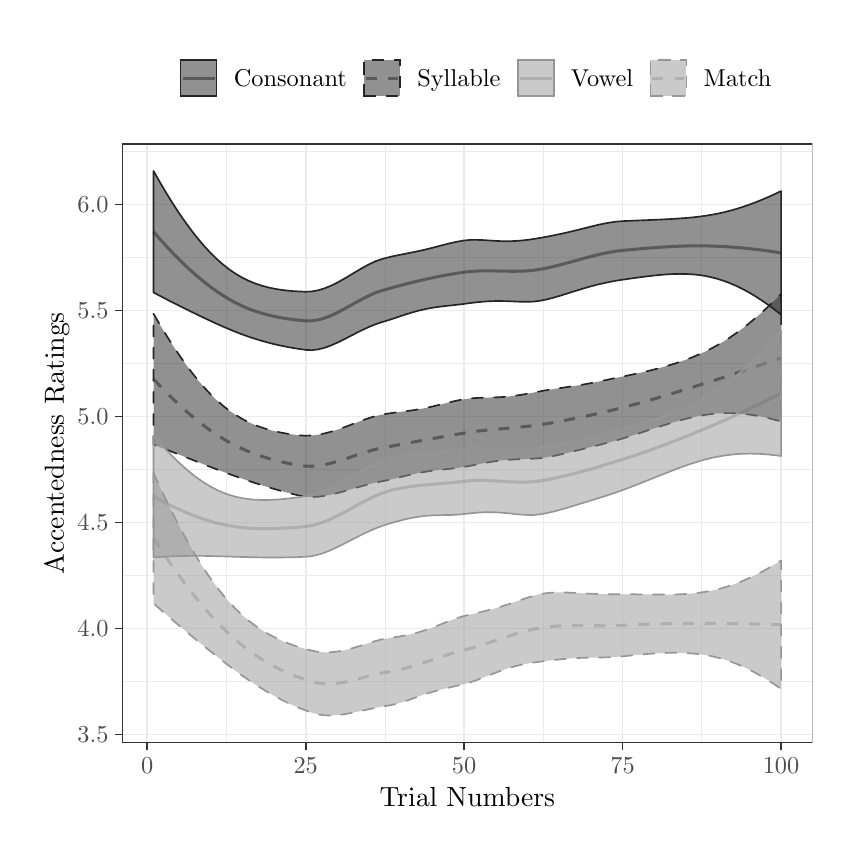
\begin{tikzpicture}[x=1pt,y=1pt]
\definecolor{fillColor}{RGB}{255,255,255}
\path[use as bounding box,fill=fillColor,fill opacity=0.00] (0,0) rectangle (289.08,289.08);
\begin{scope}
\path[clip] (  0.00,  0.00) rectangle (289.08,289.08);
\definecolor{drawColor}{RGB}{255,255,255}
\definecolor{fillColor}{RGB}{255,255,255}

\path[draw=drawColor,line width= 0.6pt,line join=round,line cap=round,fill=fillColor] (  0.00,  0.00) rectangle (289.08,289.08);
\end{scope}
\begin{scope}
\path[clip] ( 34.16, 30.69) rectangle (283.58,247.13);
\definecolor{fillColor}{RGB}{255,255,255}

\path[fill=fillColor] ( 34.16, 30.69) rectangle (283.58,247.13);
\definecolor{drawColor}{gray}{0.92}

\path[draw=drawColor,line width= 0.3pt,line join=round] ( 34.16, 52.87) --
	(283.58, 52.87);

\path[draw=drawColor,line width= 0.3pt,line join=round] ( 34.16, 91.17) --
	(283.58, 91.17);

\path[draw=drawColor,line width= 0.3pt,line join=round] ( 34.16,129.47) --
	(283.58,129.47);

\path[draw=drawColor,line width= 0.3pt,line join=round] ( 34.16,167.77) --
	(283.58,167.77);

\path[draw=drawColor,line width= 0.3pt,line join=round] ( 34.16,206.07) --
	(283.58,206.07);

\path[draw=drawColor,line width= 0.3pt,line join=round] ( 34.16,244.37) --
	(283.58,244.37);

\path[draw=drawColor,line width= 0.3pt,line join=round] ( 71.83, 30.69) --
	( 71.83,247.13);

\path[draw=drawColor,line width= 0.3pt,line join=round] (129.09, 30.69) --
	(129.09,247.13);

\path[draw=drawColor,line width= 0.3pt,line join=round] (186.35, 30.69) --
	(186.35,247.13);

\path[draw=drawColor,line width= 0.3pt,line join=round] (243.61, 30.69) --
	(243.61,247.13);

\path[draw=drawColor,line width= 0.6pt,line join=round] ( 34.16, 33.72) --
	(283.58, 33.72);

\path[draw=drawColor,line width= 0.6pt,line join=round] ( 34.16, 72.02) --
	(283.58, 72.02);

\path[draw=drawColor,line width= 0.6pt,line join=round] ( 34.16,110.32) --
	(283.58,110.32);

\path[draw=drawColor,line width= 0.6pt,line join=round] ( 34.16,148.62) --
	(283.58,148.62);

\path[draw=drawColor,line width= 0.6pt,line join=round] ( 34.16,186.92) --
	(283.58,186.92);

\path[draw=drawColor,line width= 0.6pt,line join=round] ( 34.16,225.22) --
	(283.58,225.22);

\path[draw=drawColor,line width= 0.6pt,line join=round] ( 43.20, 30.69) --
	( 43.20,247.13);

\path[draw=drawColor,line width= 0.6pt,line join=round] (100.46, 30.69) --
	(100.46,247.13);

\path[draw=drawColor,line width= 0.6pt,line join=round] (157.72, 30.69) --
	(157.72,247.13);

\path[draw=drawColor,line width= 0.6pt,line join=round] (214.98, 30.69) --
	(214.98,247.13);

\path[draw=drawColor,line width= 0.6pt,line join=round] (272.24, 30.69) --
	(272.24,247.13);
\definecolor{drawColor}{RGB}{37,37,37}

\path[draw=drawColor,draw opacity=0.50,line width= 1.1pt,line join=round] ( 45.49,215.33) --
	( 47.78,212.70) --
	( 50.07,210.17) --
	( 52.36,207.73) --
	( 54.66,205.39) --
	( 56.95,203.16) --
	( 59.24,201.04) --
	( 61.53,199.04) --
	( 63.82,197.15) --
	( 66.11,195.38) --
	( 68.40,193.73) --
	( 70.69,192.22) --
	( 72.98,190.83) --
	( 75.27,189.59) --
	( 77.56,188.49) --
	( 79.85,187.52) --
	( 82.14,186.67) --
	( 84.43,185.93) --
	( 86.72,185.30) --
	( 89.01,184.76) --
	( 91.30,184.31) --
	( 93.59,183.93) --
	( 95.88,183.62) --
	( 98.17,183.36) --
	(100.46,183.15) --
	(102.75,183.16) --
	(105.04,183.51) --
	(107.33,184.16) --
	(109.62,185.05) --
	(111.91,186.13) --
	(114.21,187.32) --
	(116.50,188.59) --
	(118.79,189.88) --
	(121.08,191.12) --
	(123.37,192.27) --
	(125.66,193.27) --
	(127.95,194.06) --
	(130.24,194.71) --
	(132.53,195.35) --
	(134.82,195.97) --
	(137.11,196.57) --
	(139.40,197.14) --
	(141.69,197.69) --
	(143.98,198.21) --
	(146.27,198.71) --
	(148.56,199.18) --
	(150.85,199.61) --
	(153.14,200.02) --
	(155.43,200.39) --
	(157.72,200.72) --
	(160.01,200.98) --
	(162.30,201.13) --
	(164.59,201.20) --
	(166.88,201.20) --
	(169.17,201.16) --
	(171.47,201.11) --
	(173.76,201.07) --
	(176.05,201.06) --
	(178.34,201.09) --
	(180.63,201.21) --
	(182.92,201.42) --
	(185.21,201.76) --
	(187.50,202.20) --
	(189.79,202.71) --
	(192.08,203.28) --
	(194.37,203.89) --
	(196.66,204.52) --
	(198.95,205.16) --
	(201.24,205.79) --
	(203.53,206.40) --
	(205.82,206.98) --
	(208.11,207.50) --
	(210.40,207.95) --
	(212.69,208.32) --
	(214.98,208.59) --
	(217.27,208.80) --
	(219.56,209.01) --
	(221.85,209.22) --
	(224.14,209.41) --
	(226.43,209.59) --
	(228.73,209.75) --
	(231.02,209.89) --
	(233.31,210.02) --
	(235.60,210.12) --
	(237.89,210.19) --
	(240.18,210.24) --
	(242.47,210.25) --
	(244.76,210.23) --
	(247.05,210.17) --
	(249.34,210.09) --
	(251.63,209.97) --
	(253.92,209.83) --
	(256.21,209.65) --
	(258.50,209.45) --
	(260.79,209.22) --
	(263.08,208.97) --
	(265.37,208.68) --
	(267.66,208.38) --
	(269.95,208.05) --
	(272.24,207.70);

\path[draw=drawColor,draw opacity=0.50,line width= 1.1pt,dash pattern=on 4pt off 4pt ,line join=round] ( 45.49,162.06) --
	( 47.78,159.65) --
	( 50.07,157.31) --
	( 52.36,155.05) --
	( 54.66,152.87) --
	( 56.95,150.79) --
	( 59.24,148.80) --
	( 61.53,146.91) --
	( 63.82,145.13) --
	( 66.11,143.46) --
	( 68.40,141.91) --
	( 70.69,140.48) --
	( 72.98,139.17) --
	( 75.27,137.98) --
	( 77.56,136.90) --
	( 79.85,135.92) --
	( 82.14,135.03) --
	( 84.43,134.23) --
	( 86.72,133.51) --
	( 89.01,132.86) --
	( 91.30,132.28) --
	( 93.59,131.76) --
	( 95.88,131.30) --
	( 98.17,130.88) --
	(100.46,130.62) --
	(102.75,130.60) --
	(105.04,130.80) --
	(107.33,131.18) --
	(109.62,131.71) --
	(111.91,132.35) --
	(114.21,133.07) --
	(116.50,133.84) --
	(118.79,134.62) --
	(121.08,135.38) --
	(123.37,136.08) --
	(125.66,136.70) --
	(127.95,137.20) --
	(130.24,137.63) --
	(132.53,138.05) --
	(134.82,138.48) --
	(137.11,138.91) --
	(139.40,139.33) --
	(141.69,139.75) --
	(143.98,140.17) --
	(146.27,140.59) --
	(148.56,141.00) --
	(150.85,141.40) --
	(153.14,141.80) --
	(155.43,142.20) --
	(157.72,142.59) --
	(160.01,142.94) --
	(162.30,143.25) --
	(164.59,143.52) --
	(166.88,143.76) --
	(169.17,143.97) --
	(171.47,144.17) --
	(173.76,144.37) --
	(176.05,144.57) --
	(178.34,144.79) --
	(180.63,145.03) --
	(182.92,145.30) --
	(185.21,145.60) --
	(187.50,145.96) --
	(189.79,146.36) --
	(192.08,146.77) --
	(194.37,147.20) --
	(196.66,147.65) --
	(198.95,148.11) --
	(201.24,148.59) --
	(203.53,149.09) --
	(205.82,149.61) --
	(208.11,150.13) --
	(210.40,150.68) --
	(212.69,151.24) --
	(214.98,151.81) --
	(217.27,152.40) --
	(219.56,153.01) --
	(221.85,153.64) --
	(224.14,154.29) --
	(226.43,154.95) --
	(228.73,155.62) --
	(231.02,156.31) --
	(233.31,157.01) --
	(235.60,157.71) --
	(237.89,158.42) --
	(240.18,159.14) --
	(242.47,159.86) --
	(244.76,160.58) --
	(247.05,161.30) --
	(249.34,162.03) --
	(251.63,162.77) --
	(253.92,163.51) --
	(256.21,164.27) --
	(258.50,165.03) --
	(260.79,165.80) --
	(263.08,166.58) --
	(265.37,167.37) --
	(267.66,168.17) --
	(269.95,168.98) --
	(272.24,169.81);
\definecolor{drawColor}{RGB}{150,150,150}

\path[draw=drawColor,draw opacity=0.50,line width= 1.1pt,line join=round] ( 45.49,119.69) --
	( 47.78,118.44) --
	( 50.07,117.24) --
	( 52.36,116.10) --
	( 54.66,115.03) --
	( 56.95,114.02) --
	( 59.24,113.07) --
	( 61.53,112.20) --
	( 63.82,111.41) --
	( 66.11,110.69) --
	( 68.40,110.07) --
	( 70.69,109.53) --
	( 72.98,109.08) --
	( 75.27,108.72) --
	( 77.56,108.44) --
	( 79.85,108.24) --
	( 82.14,108.10) --
	( 84.43,108.03) --
	( 86.72,108.02) --
	( 89.01,108.06) --
	( 91.30,108.15) --
	( 93.59,108.28) --
	( 95.88,108.43) --
	( 98.17,108.62) --
	(100.46,108.83) --
	(102.75,109.18) --
	(105.04,109.78) --
	(107.33,110.58) --
	(109.62,111.56) --
	(111.91,112.66) --
	(114.21,113.86) --
	(116.50,115.11) --
	(118.79,116.38) --
	(121.08,117.62) --
	(123.37,118.80) --
	(125.66,119.88) --
	(127.95,120.83) --
	(130.24,121.59) --
	(132.53,122.19) --
	(134.82,122.69) --
	(137.11,123.09) --
	(139.40,123.42) --
	(141.69,123.69) --
	(143.98,123.91) --
	(146.27,124.10) --
	(148.56,124.28) --
	(150.85,124.46) --
	(153.14,124.66) --
	(155.43,124.89) --
	(157.72,125.16) --
	(160.01,125.40) --
	(162.30,125.50) --
	(164.59,125.50) --
	(166.88,125.42) --
	(169.17,125.30) --
	(171.47,125.15) --
	(173.76,125.01) --
	(176.05,124.90) --
	(178.34,124.85) --
	(180.63,124.88) --
	(182.92,125.03) --
	(185.21,125.32) --
	(187.50,125.71) --
	(189.79,126.15) --
	(192.08,126.64) --
	(194.37,127.16) --
	(196.66,127.73) --
	(198.95,128.32) --
	(201.24,128.95) --
	(203.53,129.60) --
	(205.82,130.27) --
	(208.11,130.96) --
	(210.40,131.67) --
	(212.69,132.38) --
	(214.98,133.10) --
	(217.27,133.83) --
	(219.56,134.58) --
	(221.85,135.36) --
	(224.14,136.16) --
	(226.43,136.97) --
	(228.73,137.81) --
	(231.02,138.67) --
	(233.31,139.55) --
	(235.60,140.45) --
	(237.89,141.36) --
	(240.18,142.29) --
	(242.47,143.23) --
	(244.76,144.19) --
	(247.05,145.16) --
	(249.34,146.15) --
	(251.63,147.15) --
	(253.92,148.17) --
	(256.21,149.21) --
	(258.50,150.27) --
	(260.79,151.35) --
	(263.08,152.44) --
	(265.37,153.55) --
	(267.66,154.68) --
	(269.95,155.83) --
	(272.24,157.00);

\path[draw=drawColor,draw opacity=0.50,line width= 1.1pt,dash pattern=on 4pt off 4pt ,line join=round] ( 45.49,104.65) --
	( 47.78,101.10) --
	( 50.07, 97.66) --
	( 52.36, 94.32) --
	( 54.66, 91.11) --
	( 56.95, 88.01) --
	( 59.24, 85.03) --
	( 61.53, 82.17) --
	( 63.82, 79.44) --
	( 66.11, 76.83) --
	( 68.40, 74.36) --
	( 70.69, 72.02) --
	( 72.98, 69.82) --
	( 75.27, 67.76) --
	( 77.56, 65.85) --
	( 79.85, 64.08) --
	( 82.14, 62.44) --
	( 84.43, 60.94) --
	( 86.72, 59.55) --
	( 89.01, 58.28) --
	( 91.30, 57.12) --
	( 93.59, 56.06) --
	( 95.88, 55.10) --
	( 98.17, 54.23) --
	(100.46, 53.45) --
	(102.75, 52.74) --
	(105.04, 52.21) --
	(107.33, 51.97) --
	(109.62, 51.96) --
	(111.91, 52.16) --
	(114.21, 52.51) --
	(116.50, 52.99) --
	(118.79, 53.56) --
	(121.08, 54.16) --
	(123.37, 54.78) --
	(125.66, 55.36) --
	(127.95, 55.88) --
	(130.24, 56.28) --
	(132.53, 56.68) --
	(134.82, 57.18) --
	(137.11, 57.78) --
	(139.40, 58.44) --
	(141.69, 59.16) --
	(143.98, 59.91) --
	(146.27, 60.68) --
	(148.56, 61.45) --
	(150.85, 62.21) --
	(153.14, 62.93) --
	(155.43, 63.59) --
	(157.72, 64.19) --
	(160.01, 64.79) --
	(162.30, 65.45) --
	(164.59, 66.16) --
	(166.88, 66.91) --
	(169.17, 67.68) --
	(171.47, 68.44) --
	(173.76, 69.20) --
	(176.05, 69.92) --
	(178.34, 70.60) --
	(180.63, 71.21) --
	(182.92, 71.75) --
	(185.21, 72.19) --
	(187.50, 72.52) --
	(189.79, 72.75) --
	(192.08, 72.90) --
	(194.37, 72.99) --
	(196.66, 73.03) --
	(198.95, 73.04) --
	(201.24, 73.02) --
	(203.53, 72.99) --
	(205.82, 72.96) --
	(208.11, 72.95) --
	(210.40, 72.96) --
	(212.69, 73.01) --
	(214.98, 73.11) --
	(217.27, 73.24) --
	(219.56, 73.35) --
	(221.85, 73.44) --
	(224.14, 73.52) --
	(226.43, 73.59) --
	(228.73, 73.65) --
	(231.02, 73.69) --
	(233.31, 73.73) --
	(235.60, 73.76) --
	(237.89, 73.78) --
	(240.18, 73.79) --
	(242.47, 73.80) --
	(244.76, 73.80) --
	(247.05, 73.80) --
	(249.34, 73.79) --
	(251.63, 73.78) --
	(253.92, 73.76) --
	(256.21, 73.74) --
	(258.50, 73.70) --
	(260.79, 73.66) --
	(263.08, 73.61) --
	(265.37, 73.55) --
	(267.66, 73.48) --
	(269.95, 73.41) --
	(272.24, 73.32);
\definecolor{drawColor}{RGB}{37,37,37}
\definecolor{fillColor}{RGB}{37,37,37}

\path[draw=drawColor,line width= 0.6pt,line join=round,line cap=round,fill=fillColor,fill opacity=0.50] ( 45.49,237.29) --
	( 47.78,233.24) --
	( 50.07,229.36) --
	( 52.36,225.67) --
	( 54.66,222.15) --
	( 56.95,218.84) --
	( 59.24,215.72) --
	( 61.53,212.82) --
	( 63.82,210.13) --
	( 66.11,207.66) --
	( 68.40,205.42) --
	( 70.69,203.41) --
	( 72.98,201.63) --
	( 75.27,200.08) --
	( 77.56,198.74) --
	( 79.85,197.62) --
	( 82.14,196.68) --
	( 84.43,195.90) --
	( 86.72,195.27) --
	( 89.01,194.77) --
	( 91.30,194.39) --
	( 93.59,194.10) --
	( 95.88,193.89) --
	( 98.17,193.75) --
	(100.46,193.66) --
	(102.75,193.77) --
	(105.04,194.20) --
	(107.33,194.91) --
	(109.62,195.85) --
	(111.91,196.98) --
	(114.21,198.26) --
	(116.50,199.61) --
	(118.79,201.00) --
	(121.08,202.34) --
	(123.37,203.58) --
	(125.66,204.65) --
	(127.95,205.46) --
	(130.24,206.07) --
	(132.53,206.60) --
	(134.82,207.06) --
	(137.11,207.51) --
	(139.40,207.96) --
	(141.69,208.45) --
	(143.98,208.97) --
	(146.27,209.54) --
	(148.56,210.14) --
	(150.85,210.74) --
	(153.14,211.30) --
	(155.43,211.79) --
	(157.72,212.18) --
	(160.01,212.39) --
	(162.30,212.41) --
	(164.59,212.32) --
	(166.88,212.18) --
	(169.17,212.03) --
	(171.47,211.93) --
	(173.76,211.91) --
	(176.05,211.99) --
	(178.34,212.15) --
	(180.63,212.41) --
	(182.92,212.73) --
	(185.21,213.12) --
	(187.50,213.53) --
	(189.79,213.98) --
	(192.08,214.45) --
	(194.37,214.95) --
	(196.66,215.49) --
	(198.95,216.05) --
	(201.24,216.62) --
	(203.53,217.19) --
	(205.82,217.75) --
	(208.11,218.25) --
	(210.40,218.67) --
	(212.69,218.99) --
	(214.98,219.17) --
	(217.27,219.27) --
	(219.56,219.37) --
	(221.85,219.46) --
	(224.14,219.55) --
	(226.43,219.65) --
	(228.73,219.75) --
	(231.02,219.86) --
	(233.31,219.99) --
	(235.60,220.14) --
	(237.89,220.31) --
	(240.18,220.52) --
	(242.47,220.78) --
	(244.76,221.08) --
	(247.05,221.45) --
	(249.34,221.89) --
	(251.63,222.39) --
	(253.92,222.97) --
	(256.21,223.62) --
	(258.50,224.35) --
	(260.79,225.14) --
	(263.08,226.00) --
	(265.37,226.92) --
	(267.66,227.90) --
	(269.95,228.94) --
	(272.24,230.04) --
	(272.24,185.36) --
	(269.95,187.16) --
	(267.66,188.86) --
	(265.37,190.45) --
	(263.08,191.94) --
	(260.79,193.31) --
	(258.50,194.56) --
	(256.21,195.69) --
	(253.92,196.69) --
	(251.63,197.56) --
	(249.34,198.29) --
	(247.05,198.90) --
	(244.76,199.37) --
	(242.47,199.72) --
	(240.18,199.95) --
	(237.89,200.07) --
	(235.60,200.10) --
	(233.31,200.05) --
	(231.02,199.93) --
	(228.73,199.75) --
	(226.43,199.52) --
	(224.14,199.26) --
	(221.85,198.97) --
	(219.56,198.66) --
	(217.27,198.34) --
	(214.98,198.01) --
	(212.69,197.65) --
	(210.40,197.23) --
	(208.11,196.74) --
	(205.82,196.21) --
	(203.53,195.61) --
	(201.24,194.96) --
	(198.95,194.27) --
	(196.66,193.55) --
	(194.37,192.83) --
	(192.08,192.11) --
	(189.79,191.45) --
	(187.50,190.87) --
	(185.21,190.40) --
	(182.92,190.11) --
	(180.63,190.01) --
	(178.34,190.03) --
	(176.05,190.13) --
	(173.76,190.23) --
	(171.47,190.29) --
	(169.17,190.30) --
	(166.88,190.22) --
	(164.59,190.07) --
	(162.30,189.85) --
	(160.01,189.58) --
	(157.72,189.27) --
	(155.43,188.98) --
	(153.14,188.73) --
	(150.85,188.49) --
	(148.56,188.21) --
	(146.27,187.87) --
	(143.98,187.45) --
	(141.69,186.93) --
	(139.40,186.32) --
	(137.11,185.62) --
	(134.82,184.87) --
	(132.53,184.10) --
	(130.24,183.35) --
	(127.95,182.65) --
	(125.66,181.89) --
	(123.37,180.96) --
	(121.08,179.90) --
	(118.79,178.76) --
	(116.50,177.57) --
	(114.21,176.39) --
	(111.91,175.27) --
	(109.62,174.25) --
	(107.33,173.42) --
	(105.04,172.83) --
	(102.75,172.54) --
	(100.46,172.64) --
	( 98.17,172.97) --
	( 95.88,173.34) --
	( 93.59,173.75) --
	( 91.30,174.22) --
	( 89.01,174.74) --
	( 86.72,175.32) --
	( 84.43,175.96) --
	( 82.14,176.66) --
	( 79.85,177.41) --
	( 77.56,178.23) --
	( 75.27,179.10) --
	( 72.98,180.04) --
	( 70.69,181.02) --
	( 68.40,182.04) --
	( 66.11,183.09) --
	( 63.82,184.16) --
	( 61.53,185.26) --
	( 59.24,186.37) --
	( 56.95,187.49) --
	( 54.66,188.64) --
	( 52.36,189.80) --
	( 50.07,190.97) --
	( 47.78,192.17) --
	( 45.49,193.38) --
	cycle;

\path[draw=drawColor,line width= 0.6pt,dash pattern=on 4pt off 4pt ,line join=round,line cap=round,fill=fillColor,fill opacity=0.50] ( 45.49,185.70) --
	( 47.78,181.77) --
	( 50.07,177.99) --
	( 52.36,174.37) --
	( 54.66,170.92) --
	( 56.95,167.65) --
	( 59.24,164.57) --
	( 61.53,161.70) --
	( 63.82,159.03) --
	( 66.11,156.59) --
	( 68.40,154.37) --
	( 70.69,152.37) --
	( 72.98,150.61) --
	( 75.27,149.05) --
	( 77.56,147.69) --
	( 79.85,146.51) --
	( 82.14,145.50) --
	( 84.43,144.64) --
	( 86.72,143.92) --
	( 89.01,143.31) --
	( 91.30,142.81) --
	( 93.59,142.39) --
	( 95.88,142.05) --
	( 98.17,141.77) --
	(100.46,141.63) --
	(102.75,141.72) --
	(105.04,142.01) --
	(107.33,142.47) --
	(109.62,143.08) --
	(111.91,143.81) --
	(114.21,144.62) --
	(116.50,145.49) --
	(118.79,146.37) --
	(121.08,147.24) --
	(123.37,148.03) --
	(125.66,148.72) --
	(127.95,149.25) --
	(130.24,149.64) --
	(132.53,149.96) --
	(134.82,150.25) --
	(137.11,150.55) --
	(139.40,150.87) --
	(141.69,151.25) --
	(143.98,151.69) --
	(146.27,152.19) --
	(148.56,152.75) --
	(150.85,153.32) --
	(153.14,153.88) --
	(155.43,154.39) --
	(157.72,154.82) --
	(160.01,155.11) --
	(162.30,155.28) --
	(164.59,155.37) --
	(166.88,155.43) --
	(169.17,155.50) --
	(171.47,155.61) --
	(173.76,155.80) --
	(176.05,156.07) --
	(178.34,156.41) --
	(180.63,156.81) --
	(182.92,157.25) --
	(185.21,157.68) --
	(187.50,158.09) --
	(189.79,158.46) --
	(192.08,158.80) --
	(194.37,159.13) --
	(196.66,159.46) --
	(198.95,159.82) --
	(201.24,160.21) --
	(203.53,160.63) --
	(205.82,161.08) --
	(208.11,161.56) --
	(210.40,162.05) --
	(212.69,162.54) --
	(214.98,163.01) --
	(217.27,163.48) --
	(219.56,163.97) --
	(221.85,164.48) --
	(224.14,165.02) --
	(226.43,165.59) --
	(228.73,166.20) --
	(231.02,166.85) --
	(233.31,167.54) --
	(235.60,168.29) --
	(237.89,169.11) --
	(240.18,169.99) --
	(242.47,170.95) --
	(244.76,172.00) --
	(247.05,173.15) --
	(249.34,174.40) --
	(251.63,175.76) --
	(253.92,177.23) --
	(256.21,178.82) --
	(258.50,180.51) --
	(260.79,182.32) --
	(263.08,184.23) --
	(265.37,186.25) --
	(267.66,188.36) --
	(269.95,190.57) --
	(272.24,192.87) --
	(272.24,146.75) --
	(269.95,147.40) --
	(267.66,147.98) --
	(265.37,148.49) --
	(263.08,148.92) --
	(260.79,149.27) --
	(258.50,149.54) --
	(256.21,149.71) --
	(253.92,149.79) --
	(251.63,149.78) --
	(249.34,149.67) --
	(247.05,149.46) --
	(244.76,149.15) --
	(242.47,148.76) --
	(240.18,148.28) --
	(237.89,147.74) --
	(235.60,147.13) --
	(233.31,146.47) --
	(231.02,145.77) --
	(228.73,145.05) --
	(226.43,144.31) --
	(224.14,143.56) --
	(221.85,142.80) --
	(219.56,142.06) --
	(217.27,141.33) --
	(214.98,140.61) --
	(212.69,139.94) --
	(210.40,139.31) --
	(208.11,138.71) --
	(205.82,138.13) --
	(203.53,137.55) --
	(201.24,136.98) --
	(198.95,136.41) --
	(196.66,135.84) --
	(194.37,135.28) --
	(192.08,134.74) --
	(189.79,134.26) --
	(187.50,133.83) --
	(185.21,133.53) --
	(182.92,133.34) --
	(180.63,133.24) --
	(178.34,133.16) --
	(176.05,133.08) --
	(173.76,132.94) --
	(171.47,132.73) --
	(169.17,132.45) --
	(166.88,132.09) --
	(164.59,131.67) --
	(162.30,131.22) --
	(160.01,130.78) --
	(157.72,130.36) --
	(155.43,130.01) --
	(153.14,129.73) --
	(150.85,129.49) --
	(148.56,129.25) --
	(146.27,128.98) --
	(143.98,128.65) --
	(141.69,128.26) --
	(139.40,127.79) --
	(137.11,127.27) --
	(134.82,126.71) --
	(132.53,126.14) --
	(130.24,125.61) --
	(127.95,125.15) --
	(125.66,124.68) --
	(123.37,124.13) --
	(121.08,123.51) --
	(118.79,122.86) --
	(116.50,122.18) --
	(114.21,121.52) --
	(111.91,120.89) --
	(109.62,120.34) --
	(107.33,119.89) --
	(105.04,119.59) --
	(102.75,119.48) --
	(100.46,119.60) --
	( 98.17,119.99) --
	( 95.88,120.54) --
	( 93.59,121.13) --
	( 91.30,121.75) --
	( 89.01,122.41) --
	( 86.72,123.10) --
	( 84.43,123.81) --
	( 82.14,124.56) --
	( 79.85,125.32) --
	( 77.56,126.11) --
	( 75.27,126.92) --
	( 72.98,127.74) --
	( 70.69,128.58) --
	( 68.40,129.45) --
	( 66.11,130.33) --
	( 63.82,131.22) --
	( 61.53,132.12) --
	( 59.24,133.02) --
	( 56.95,133.93) --
	( 54.66,134.83) --
	( 52.36,135.73) --
	( 50.07,136.63) --
	( 47.78,137.52) --
	( 45.49,138.41) --
	cycle;
\definecolor{drawColor}{gray}{0.59}
\definecolor{fillColor}{RGB}{150,150,150}

\path[draw=drawColor,line width= 0.6pt,line join=round,line cap=round,fill=fillColor,fill opacity=0.50] ( 45.49,141.72) --
	( 47.78,139.07) --
	( 50.07,136.54) --
	( 52.36,134.16) --
	( 54.66,131.92) --
	( 56.95,129.84) --
	( 59.24,127.92) --
	( 61.53,126.18) --
	( 63.82,124.61) --
	( 66.11,123.23) --
	( 68.40,122.03) --
	( 70.69,121.02) --
	( 72.98,120.20) --
	( 75.27,119.55) --
	( 77.56,119.06) --
	( 79.85,118.72) --
	( 82.14,118.51) --
	( 84.43,118.41) --
	( 86.72,118.41) --
	( 89.01,118.50) --
	( 91.30,118.66) --
	( 93.59,118.88) --
	( 95.88,119.15) --
	( 98.17,119.45) --
	(100.46,119.78) --
	(102.75,120.23) --
	(105.04,120.90) --
	(107.33,121.76) --
	(109.62,122.78) --
	(111.91,123.93) --
	(114.21,125.18) --
	(116.50,126.51) --
	(118.79,127.86) --
	(121.08,129.20) --
	(123.37,130.48) --
	(125.66,131.65) --
	(127.95,132.65) --
	(130.24,133.43) --
	(132.53,133.98) --
	(134.82,134.35) --
	(137.11,134.60) --
	(139.40,134.78) --
	(141.69,134.95) --
	(143.98,135.13) --
	(146.27,135.36) --
	(148.56,135.64) --
	(150.85,135.96) --
	(153.14,136.32) --
	(155.43,136.67) --
	(157.72,137.00) --
	(160.01,137.19) --
	(162.30,137.19) --
	(164.59,137.05) --
	(166.88,136.85) --
	(169.17,136.65) --
	(171.47,136.50) --
	(173.76,136.42) --
	(176.05,136.45) --
	(178.34,136.57) --
	(180.63,136.78) --
	(182.92,137.07) --
	(185.21,137.41) --
	(187.50,137.77) --
	(189.79,138.13) --
	(192.08,138.50) --
	(194.37,138.90) --
	(196.66,139.34) --
	(198.95,139.83) --
	(201.24,140.37) --
	(203.53,140.97) --
	(205.82,141.60) --
	(208.11,142.26) --
	(210.40,142.93) --
	(212.69,143.58) --
	(214.98,144.20) --
	(217.27,144.80) --
	(219.56,145.43) --
	(221.85,146.09) --
	(224.14,146.77) --
	(226.43,147.49) --
	(228.73,148.25) --
	(231.02,149.06) --
	(233.31,149.93) --
	(235.60,150.85) --
	(237.89,151.85) --
	(240.18,152.93) --
	(242.47,154.09) --
	(244.76,155.36) --
	(247.05,156.74) --
	(249.34,158.23) --
	(251.63,159.85) --
	(253.92,161.58) --
	(256.21,163.45) --
	(258.50,165.43) --
	(260.79,167.54) --
	(263.08,169.76) --
	(265.37,172.09) --
	(267.66,174.53) --
	(269.95,177.07) --
	(272.24,179.72) --
	(272.24,134.29) --
	(269.95,134.59) --
	(267.66,134.84) --
	(265.37,135.01) --
	(263.08,135.12) --
	(260.79,135.16) --
	(258.50,135.11) --
	(256.21,134.98) --
	(253.92,134.76) --
	(251.63,134.46) --
	(249.34,134.06) --
	(247.05,133.58) --
	(244.76,133.01) --
	(242.47,132.36) --
	(240.18,131.65) --
	(237.89,130.87) --
	(235.60,130.04) --
	(233.31,129.18) --
	(231.02,128.28) --
	(228.73,127.37) --
	(226.43,126.46) --
	(224.14,125.54) --
	(221.85,124.62) --
	(219.56,123.73) --
	(217.27,122.85) --
	(214.98,121.99) --
	(212.69,121.18) --
	(210.40,120.41) --
	(208.11,119.66) --
	(205.82,118.94) --
	(203.53,118.23) --
	(201.24,117.53) --
	(198.95,116.82) --
	(196.66,116.12) --
	(194.37,115.43) --
	(192.08,114.77) --
	(189.79,114.17) --
	(187.50,113.65) --
	(185.21,113.23) --
	(182.92,113.00) --
	(180.63,112.99) --
	(178.34,113.13) --
	(176.05,113.35) --
	(173.76,113.59) --
	(171.47,113.80) --
	(169.17,113.94) --
	(166.88,113.99) --
	(164.59,113.95) --
	(162.30,113.81) --
	(160.01,113.60) --
	(157.72,113.33) --
	(155.43,113.11) --
	(153.14,113.00) --
	(150.85,112.96) --
	(148.56,112.93) --
	(146.27,112.85) --
	(143.98,112.69) --
	(141.69,112.43) --
	(139.40,112.06) --
	(137.11,111.58) --
	(134.82,111.02) --
	(132.53,110.40) --
	(130.24,109.75) --
	(127.95,109.00) --
	(125.66,108.12) --
	(123.37,107.13) --
	(121.08,106.05) --
	(118.79,104.90) --
	(116.50,103.72) --
	(114.21,102.54) --
	(111.91,101.40) --
	(109.62,100.34) --
	(107.33, 99.40) --
	(105.04, 98.65) --
	(102.75, 98.13) --
	(100.46, 97.88) --
	( 98.17, 97.79) --
	( 95.88, 97.72) --
	( 93.59, 97.67) --
	( 91.30, 97.64) --
	( 89.01, 97.63) --
	( 86.72, 97.63) --
	( 84.43, 97.66) --
	( 82.14, 97.70) --
	( 79.85, 97.75) --
	( 77.56, 97.82) --
	( 75.27, 97.88) --
	( 72.98, 97.95) --
	( 70.69, 98.03) --
	( 68.40, 98.10) --
	( 66.11, 98.16) --
	( 63.82, 98.20) --
	( 61.53, 98.22) --
	( 59.24, 98.22) --
	( 56.95, 98.19) --
	( 54.66, 98.14) --
	( 52.36, 98.05) --
	( 50.07, 97.94) --
	( 47.78, 97.81) --
	( 45.49, 97.65) --
	cycle;

\path[draw=drawColor,line width= 0.6pt,dash pattern=on 4pt off 4pt ,line join=round,line cap=round,fill=fillColor,fill opacity=0.50] ( 45.49,128.28) --
	( 47.78,123.20) --
	( 50.07,118.31) --
	( 52.36,113.62) --
	( 54.66,109.13) --
	( 56.95,104.85) --
	( 59.24,100.80) --
	( 61.53, 96.96) --
	( 63.82, 93.36) --
	( 66.11, 89.99) --
	( 68.40, 86.87) --
	( 70.69, 83.98) --
	( 72.98, 81.33) --
	( 75.27, 78.93) --
	( 77.56, 76.76) --
	( 79.85, 74.81) --
	( 82.14, 73.06) --
	( 84.43, 71.50) --
	( 86.72, 70.12) --
	( 89.01, 68.88) --
	( 91.30, 67.79) --
	( 93.59, 66.82) --
	( 95.88, 65.97) --
	( 98.17, 65.21) --
	(100.46, 64.54) --
	(102.75, 63.96) --
	(105.04, 63.53) --
	(107.33, 63.36) --
	(109.62, 63.40) --
	(111.91, 63.65) --
	(114.21, 64.06) --
	(116.50, 64.62) --
	(118.79, 65.28) --
	(121.08, 66.00) --
	(123.37, 66.74) --
	(125.66, 67.43) --
	(127.95, 68.03) --
	(130.24, 68.46) --
	(132.53, 68.80) --
	(134.82, 69.18) --
	(137.11, 69.61) --
	(139.40, 70.12) --
	(141.69, 70.74) --
	(143.98, 71.46) --
	(146.27, 72.29) --
	(148.56, 73.19) --
	(150.85, 74.12) --
	(153.14, 75.02) --
	(155.43, 75.83) --
	(157.72, 76.49) --
	(160.01, 77.04) --
	(162.30, 77.57) --
	(164.59, 78.12) --
	(166.88, 78.69) --
	(169.17, 79.31) --
	(171.47, 80.00) --
	(173.76, 80.75) --
	(176.05, 81.54) --
	(178.34, 82.34) --
	(180.63, 83.12) --
	(182.92, 83.82) --
	(185.21, 84.38) --
	(187.50, 84.76) --
	(189.79, 84.95) --
	(192.08, 85.01) --
	(194.37, 84.98) --
	(196.66, 84.89) --
	(198.95, 84.77) --
	(201.24, 84.64) --
	(203.53, 84.53) --
	(205.82, 84.44) --
	(208.11, 84.38) --
	(210.40, 84.34) --
	(212.69, 84.32) --
	(214.98, 84.33) --
	(217.27, 84.33) --
	(219.56, 84.32) --
	(221.85, 84.30) --
	(224.14, 84.27) --
	(226.43, 84.25) --
	(228.73, 84.23) --
	(231.02, 84.23) --
	(233.31, 84.26) --
	(235.60, 84.33) --
	(237.89, 84.45) --
	(240.18, 84.63) --
	(242.47, 84.88) --
	(244.76, 85.21) --
	(247.05, 85.63) --
	(249.34, 86.14) --
	(251.63, 86.76) --
	(253.92, 87.48) --
	(256.21, 88.30) --
	(258.50, 89.21) --
	(260.79, 90.23) --
	(263.08, 91.33) --
	(265.37, 92.51) --
	(267.66, 93.78) --
	(269.95, 95.13) --
	(272.24, 96.54) --
	(272.24, 50.10) --
	(269.95, 51.69) --
	(267.66, 53.19) --
	(265.37, 54.59) --
	(263.08, 55.89) --
	(260.79, 57.09) --
	(258.50, 58.19) --
	(256.21, 59.17) --
	(253.92, 60.05) --
	(251.63, 60.80) --
	(249.34, 61.45) --
	(247.05, 61.98) --
	(244.76, 62.40) --
	(242.47, 62.72) --
	(240.18, 62.95) --
	(237.89, 63.10) --
	(235.60, 63.18) --
	(233.31, 63.20) --
	(231.02, 63.16) --
	(228.73, 63.07) --
	(226.43, 62.94) --
	(224.14, 62.78) --
	(221.85, 62.59) --
	(219.56, 62.38) --
	(217.27, 62.15) --
	(214.98, 61.90) --
	(212.69, 61.70) --
	(210.40, 61.58) --
	(208.11, 61.52) --
	(205.82, 61.48) --
	(203.53, 61.45) --
	(201.24, 61.40) --
	(198.95, 61.31) --
	(196.66, 61.18) --
	(194.37, 61.01) --
	(192.08, 60.79) --
	(189.79, 60.55) --
	(187.50, 60.28) --
	(185.21, 60.00) --
	(182.92, 59.68) --
	(180.63, 59.31) --
	(178.34, 58.86) --
	(176.05, 58.31) --
	(173.76, 57.65) --
	(171.47, 56.89) --
	(169.17, 56.04) --
	(166.88, 55.13) --
	(164.59, 54.21) --
	(162.30, 53.33) --
	(160.01, 52.54) --
	(157.72, 51.89) --
	(155.43, 51.36) --
	(153.14, 50.83) --
	(150.85, 50.29) --
	(148.56, 49.71) --
	(146.27, 49.07) --
	(143.98, 48.36) --
	(141.69, 47.58) --
	(139.40, 46.76) --
	(137.11, 45.94) --
	(134.82, 45.19) --
	(132.53, 44.56) --
	(130.24, 44.10) --
	(127.95, 43.73) --
	(125.66, 43.30) --
	(123.37, 42.82) --
	(121.08, 42.33) --
	(118.79, 41.83) --
	(116.50, 41.37) --
	(114.21, 40.97) --
	(111.91, 40.67) --
	(109.62, 40.52) --
	(107.33, 40.58) --
	(105.04, 40.89) --
	(102.75, 41.52) --
	(100.46, 42.35) --
	( 98.17, 43.25) --
	( 95.88, 44.24) --
	( 93.59, 45.31) --
	( 91.30, 46.45) --
	( 89.01, 47.68) --
	( 86.72, 48.99) --
	( 84.43, 50.37) --
	( 82.14, 51.82) --
	( 79.85, 53.34) --
	( 77.56, 54.93) --
	( 75.27, 56.59) --
	( 72.98, 58.30) --
	( 70.69, 60.06) --
	( 68.40, 61.85) --
	( 66.11, 63.67) --
	( 63.82, 65.51) --
	( 61.53, 67.37) --
	( 59.24, 69.26) --
	( 56.95, 71.16) --
	( 54.66, 73.08) --
	( 52.36, 75.03) --
	( 50.07, 77.00) --
	( 47.78, 79.00) --
	( 45.49, 81.03) --
	cycle;
\definecolor{drawColor}{gray}{0.20}

\path[draw=drawColor,line width= 0.6pt,line join=round,line cap=round] ( 34.16, 30.69) rectangle (283.58,247.13);
\end{scope}
\begin{scope}
\path[clip] (  0.00,  0.00) rectangle (289.08,289.08);
\definecolor{drawColor}{gray}{0.30}

\node[text=drawColor,anchor=base east,inner sep=0pt, outer sep=0pt, scale=  0.88] at ( 29.21, 30.69) {3.5};

\node[text=drawColor,anchor=base east,inner sep=0pt, outer sep=0pt, scale=  0.88] at ( 29.21, 68.99) {4.0};

\node[text=drawColor,anchor=base east,inner sep=0pt, outer sep=0pt, scale=  0.88] at ( 29.21,107.29) {4.5};

\node[text=drawColor,anchor=base east,inner sep=0pt, outer sep=0pt, scale=  0.88] at ( 29.21,145.59) {5.0};

\node[text=drawColor,anchor=base east,inner sep=0pt, outer sep=0pt, scale=  0.88] at ( 29.21,183.89) {5.5};

\node[text=drawColor,anchor=base east,inner sep=0pt, outer sep=0pt, scale=  0.88] at ( 29.21,222.19) {6.0};
\end{scope}
\begin{scope}
\path[clip] (  0.00,  0.00) rectangle (289.08,289.08);
\definecolor{drawColor}{gray}{0.20}

\path[draw=drawColor,line width= 0.6pt,line join=round] ( 31.41, 33.72) --
	( 34.16, 33.72);

\path[draw=drawColor,line width= 0.6pt,line join=round] ( 31.41, 72.02) --
	( 34.16, 72.02);

\path[draw=drawColor,line width= 0.6pt,line join=round] ( 31.41,110.32) --
	( 34.16,110.32);

\path[draw=drawColor,line width= 0.6pt,line join=round] ( 31.41,148.62) --
	( 34.16,148.62);

\path[draw=drawColor,line width= 0.6pt,line join=round] ( 31.41,186.92) --
	( 34.16,186.92);

\path[draw=drawColor,line width= 0.6pt,line join=round] ( 31.41,225.22) --
	( 34.16,225.22);
\end{scope}
\begin{scope}
\path[clip] (  0.00,  0.00) rectangle (289.08,289.08);
\definecolor{drawColor}{gray}{0.20}

\path[draw=drawColor,line width= 0.6pt,line join=round] ( 43.20, 27.94) --
	( 43.20, 30.69);

\path[draw=drawColor,line width= 0.6pt,line join=round] (100.46, 27.94) --
	(100.46, 30.69);

\path[draw=drawColor,line width= 0.6pt,line join=round] (157.72, 27.94) --
	(157.72, 30.69);

\path[draw=drawColor,line width= 0.6pt,line join=round] (214.98, 27.94) --
	(214.98, 30.69);

\path[draw=drawColor,line width= 0.6pt,line join=round] (272.24, 27.94) --
	(272.24, 30.69);
\end{scope}
\begin{scope}
\path[clip] (  0.00,  0.00) rectangle (289.08,289.08);
\definecolor{drawColor}{gray}{0.30}

\node[text=drawColor,anchor=base,inner sep=0pt, outer sep=0pt, scale=  0.88] at ( 43.20, 19.68) {0};

\node[text=drawColor,anchor=base,inner sep=0pt, outer sep=0pt, scale=  0.88] at (100.46, 19.68) {25};

\node[text=drawColor,anchor=base,inner sep=0pt, outer sep=0pt, scale=  0.88] at (157.72, 19.68) {50};

\node[text=drawColor,anchor=base,inner sep=0pt, outer sep=0pt, scale=  0.88] at (214.98, 19.68) {75};

\node[text=drawColor,anchor=base,inner sep=0pt, outer sep=0pt, scale=  0.88] at (272.24, 19.68) {100};
\end{scope}
\begin{scope}
\path[clip] (  0.00,  0.00) rectangle (289.08,289.08);
\definecolor{drawColor}{RGB}{0,0,0}

\node[text=drawColor,anchor=base,inner sep=0pt, outer sep=0pt, scale=  1] at (158.87,  7.64) {Trial Numbers};
\end{scope}
\begin{scope}
\path[clip] (  0.00,  0.00) rectangle (289.08,289.08);
\definecolor{drawColor}{RGB}{0,0,0}

\node[text=drawColor,rotate= 90.00,anchor=base,inner sep=0pt, outer sep=0pt, scale=  1] at ( 13.08,138.91) {Accentedness Ratings};
\end{scope}
\begin{scope}
\path[clip] (  0.00,  0.00) rectangle (289.08,289.08);
\definecolor{fillColor}{RGB}{255,255,255}

\path[fill=fillColor] ( 43.54,258.13) rectangle (274.20,283.58);
\end{scope}
\begin{scope}
\path[clip] (  0.00,  0.00) rectangle (289.08,289.08);
\definecolor{fillColor}{RGB}{255,255,255}

\path[fill=fillColor] ( 54.54,263.63) rectangle ( 68.99,278.08);
\end{scope}
\begin{scope}
\path[clip] (  0.00,  0.00) rectangle (289.08,289.08);
\definecolor{drawColor}{RGB}{37,37,37}

\path[draw=drawColor,draw opacity=0.50,line width= 1.1pt,line join=round] ( 55.98,270.85) -- ( 67.55,270.85);
\end{scope}
\begin{scope}
\path[clip] (  0.00,  0.00) rectangle (289.08,289.08);
\definecolor{drawColor}{RGB}{37,37,37}
\definecolor{fillColor}{RGB}{37,37,37}

\path[draw=drawColor,line width= 0.6pt,line cap=rect,fill=fillColor,fill opacity=0.50] ( 55.25,264.34) rectangle ( 68.28,277.37);
\end{scope}
\begin{scope}
\path[clip] (  0.00,  0.00) rectangle (289.08,289.08);
\definecolor{fillColor}{RGB}{255,255,255}

\path[fill=fillColor] (120.85,263.63) rectangle (135.31,278.08);
\end{scope}
\begin{scope}
\path[clip] (  0.00,  0.00) rectangle (289.08,289.08);
\definecolor{drawColor}{RGB}{37,37,37}

\path[draw=drawColor,draw opacity=0.50,line width= 1.1pt,dash pattern=on 4pt off 4pt ,line join=round] (122.30,270.85) -- (133.86,270.85);
\end{scope}
\begin{scope}
\path[clip] (  0.00,  0.00) rectangle (289.08,289.08);
\definecolor{drawColor}{RGB}{37,37,37}
\definecolor{fillColor}{RGB}{37,37,37}

\path[draw=drawColor,line width= 0.6pt,dash pattern=on 4pt off 4pt ,line cap=rect,fill=fillColor,fill opacity=0.50] (121.57,264.34) rectangle (134.60,277.37);
\end{scope}
\begin{scope}
\path[clip] (  0.00,  0.00) rectangle (289.08,289.08);
\definecolor{fillColor}{RGB}{255,255,255}

\path[fill=fillColor] (176.37,263.63) rectangle (190.82,278.08);
\end{scope}
\begin{scope}
\path[clip] (  0.00,  0.00) rectangle (289.08,289.08);
\definecolor{drawColor}{RGB}{150,150,150}

\path[draw=drawColor,draw opacity=0.50,line width= 1.1pt,line join=round] (177.81,270.85) -- (189.38,270.85);
\end{scope}
\begin{scope}
\path[clip] (  0.00,  0.00) rectangle (289.08,289.08);
\definecolor{drawColor}{gray}{0.59}
\definecolor{fillColor}{RGB}{150,150,150}

\path[draw=drawColor,line width= 0.6pt,line cap=rect,fill=fillColor,fill opacity=0.50] (177.08,264.34) rectangle (190.11,277.37);
\end{scope}
\begin{scope}
\path[clip] (  0.00,  0.00) rectangle (289.08,289.08);
\definecolor{fillColor}{RGB}{255,255,255}

\path[fill=fillColor] (224.30,263.63) rectangle (238.76,278.08);
\end{scope}
\begin{scope}
\path[clip] (  0.00,  0.00) rectangle (289.08,289.08);
\definecolor{drawColor}{RGB}{150,150,150}

\path[draw=drawColor,draw opacity=0.50,line width= 1.1pt,dash pattern=on 4pt off 4pt ,line join=round] (225.75,270.85) -- (237.31,270.85);
\end{scope}
\begin{scope}
\path[clip] (  0.00,  0.00) rectangle (289.08,289.08);
\definecolor{drawColor}{gray}{0.59}
\definecolor{fillColor}{RGB}{150,150,150}

\path[draw=drawColor,line width= 0.6pt,dash pattern=on 4pt off 4pt ,line cap=rect,fill=fillColor,fill opacity=0.50] (225.02,264.34) rectangle (238.05,277.37);
\end{scope}
\begin{scope}
\path[clip] (  0.00,  0.00) rectangle (289.08,289.08);
\definecolor{drawColor}{RGB}{0,0,0}

\node[text=drawColor,anchor=base west,inner sep=0pt, outer sep=0pt, scale=  0.88] at ( 74.49,267.82) {Consonant};
\end{scope}
\begin{scope}
\path[clip] (  0.00,  0.00) rectangle (289.08,289.08);
\definecolor{drawColor}{RGB}{0,0,0}

\node[text=drawColor,anchor=base west,inner sep=0pt, outer sep=0pt, scale=  0.88] at (140.81,267.82) {Syllable};
\end{scope}
\begin{scope}
\path[clip] (  0.00,  0.00) rectangle (289.08,289.08);
\definecolor{drawColor}{RGB}{0,0,0}

\node[text=drawColor,anchor=base west,inner sep=0pt, outer sep=0pt, scale=  0.88] at (196.32,267.82) {Vowel};
\end{scope}
\begin{scope}
\path[clip] (  0.00,  0.00) rectangle (289.08,289.08);
\definecolor{drawColor}{RGB}{0,0,0}

\node[text=drawColor,anchor=base west,inner sep=0pt, outer sep=0pt, scale=  0.88] at (244.26,267.82) {Match};
\end{scope}
\end{tikzpicture}

    \caption{Ratings across Time}
    \label{fig:trial1}
  \figSpace
\end{figure}

Figure \ref{fig:trial1}, in general, confirms the findings in the previous section. That is, stimuli with segmental and structural mismatches were rated as more accented than the match stimuli, and consonant mismatches had higher ratings than the other two types of mismatches. The ratings for all stimuli gradually decreased during the first 20 to 25 trials, and then began to increase. 

\subsection{Individual Mismatches}
The analysis above showed that consonant mismatches were judged to be more accented in general. It might be too hasty to draw the conclusion that all consonant mismatches are more accented than the other two types of mismatch stimuli. As mentioned in Chapter 3, stimuli of the current study included 11 types of consonant mismatches, 5 types of vowel mismatches, and 2 types of syllable structure mismatches. The phonological context for each mismatch could have had an effect on whether the mismatch was rated as foreign accented. It is, therefore, important to further examine the possible effect of phonological context on accentedness perception.

Recall that the mismatches occurred in five contexts, namely “\textit{ask her},” “\textit{please call},” “\textit{six spoons},” “\textit{five thick},” and “\textit{small plastic}.” The following session uses context “\textit{ask her}” as an example to discuss the statistical method. Since statistical methods used for the other four contexts were the same as the one used for “\textit{ask her},” the details for these four contexts are omitted.


\subsubsection{Context 1: “\textit{Ask her}”}

For “\textit{ask her},” there were seven types of mismatch as listed on the y-axis of Figure \ref{fig:ah1}. In general, syllable mismatches such as vowel epenthesis (i.e., [æsk]$\rightarrow$[æskə]) and /ɹ/-trilling (i.e., [ɹ]$\rightarrow$[r]) received the highest ratings. Coda-deletion (i.e., [æsk]$\rightarrow$[æs]) received a relatively higher mean rating. Arithmetic mean ratings of the seven types of mismatches and the match stimuli are presented in Figure \ref{fig:ah1}, where the error bars represent the 95\% confidence intervals.

Mixed-effects linear regression models were constructed to investigate the effect of individual mismatch on accentedness. The ratings were the dependent variable. The eight types of stimuli and trial number were entered as fixed effects. Raters were entered as a random effect with the type of stimuli as the random slope. Stimuli were entered as another random effect.


\begin{figure}[h!]
  \figSpace
\centering

\begin{tikzpicture}
  \begin{axis}[
  title={Mean Accentedness Ratings},
     % xbar,
   ytick={1,2,3,4,5,6,7,8},
     y=1cm,
  bar width=0.7 cm,
  xmin=0,
  xmax=7.1,
    axis y line*=left,
   axis x line=bottom,
    tickwidth         = 1pt,
    enlarge y limits  = 0.1,
    enlarge x limits  = 0.02,
  legend style={at={(1.2,0.55)},
  anchor=north},
  legend cell align=left,
      yticklabels from table={figures/bar1/data_askher.txt}{label},
      xtick distance=2,
      every axis plot/.append style={
          xbar,
          bar shift=0pt,
          fill
        }
    ]
\addplot [fill=red,color=mycolor3,select coords between index={0}{0}] table  [x=x,y=y] {figures/bar1/data_askher.txt};
\addplot [fill=red,color=mycolor1,select coords between index={1}{1}] table  [x=x,y=y] {figures/bar1/data_askher.txt};
\addplot [fill=blue,color=mycolor3,select coords between index={2}{8}] table [x=x, y=y] {figures/bar1/data_askher.txt};
 \addplot [color=black, only marks, mark=o]
 plot [error bars/.cd, x dir = both, x explicit]
 table[x =x, y =y, x error =err]{figures/bar1/data_askher.txt};
 \end{axis}
\node[] at (6.7,7.7) {5.99};
\node[] at (6.6,6.7) {5.82};
\node[] at (6.45,5.7) {5.78};
\node[] at (6.4,4.7) {5.73};
\node[] at (6.14,3.7) {5.01};
\node[] at (5.65,2.7) {4.71};
\node[] at (5.31,1.7) {4.08};
\node[] at (5.15,0.7) {3.90};


\end{tikzpicture}
\caption{Mean Accentedness Ratings of Stimuli in “\textit{Ask her}”}
\label{fig:ah1}
\figSpace
\end{figure}

Model comparisons using likelihood ratio tests revealed that the type of stimuli contributed significantly to model fit (χ2 = 18.40, p < .01), showing that the eight types of stimuli were indeed rated differently.  Trial number was another significant contributing factor to model fit (χ2 = 7.84, p < .01), showing that the same stimulus would be considered more accented if it occurred late in the experiment. The interaction between type of stimuli and trial numbers did not contribute significantly to model fit (χ2 = 5.04, p =.66), showing that rating differences of the stimuli were consistent overtime. To further investigate the rating differences between the eight type of stimuli, Helmert-contrast-coding was implemented to create seven contrasts (Table \ref{table:contr1}).

% Table generated by Excel2LaTeX from sheet 'Sheet6'
\begin{table}[h!]
  \centering
    \figSpace
  \caption{Stimuli Contrasts}
  \label{table:contr1}%
    \begin{tabular}{lrrrrrrr}
    \toprule
 Levels & Contrast1 & Contrast2 & Contrast3 & Contrast4 & Contrast5 & Contrast6 & Contrast7 \\
    \midrule
    æ$\rightarrow$æ̞    & -0.5  & -0.333 & -0.25 & -0.2  & -0.167 & -0.143 & -0.125 \\
    Match     & 0.5   & -0.333 & -0.25 & -0.2  & -0.167 & -0.143 & -0.125 \\
    æ$\rightarrow$a     & 0     & 0.667 & -0.25 & -0.2  & -0.167 & -0.143 & -0.125 \\
    æ$\rightarrow$æ̝     & 0     & 0     & 0.75  & -0.2  & -0.167 & -0.143 & -0.125 \\
    æ$\rightarrow$ɑ     & 0     & 0     & 0     & 0.8   & -0.167 & -0.143 & -0.125 \\
    æsk$\rightarrow$æs     & 0     & 0     & 0     & 0     & 0.833 & -0.143 & -0.125 \\
    ɹ$\rightarrow$r     & 0     & 0     & 0     & 0     & 0     & 0.857 & -0.125 \\
    æsk$\rightarrow$æskə    & 0     & 0     & 0     & 0     & 0     & 0     & 0.875 \\
    \bottomrule
    \end{tabular}%
      \figSpace
\end{table}%

Helmert-contrast coding was used to achieve comparisons among the eight types of stimuli. For example, the first contrast in Table \ref{table:contr1} (i.e., Contrast1) compares ratings of [æ]$\rightarrow$[æ̞] to ratings of the match stimuli, while the second contrast (i.e., Contrast2) compares ratings of [æ]$\rightarrow$[a] to ratings of both [æ]$\rightarrow$[æ̞] and the match stimuli. Since the seven contrasts were entered into the model as fixed effect factors, model comparisons using the likelihood ratio test could show whether any of the contrasts contributed significantly to model fit. 

The full model took accentedness ratings as the dependent variable, the seven contrasts as fixed effects. Trial number and the interactions between trial number and the seven contrasts were also entered as fixed effects. Raters and stimuli were used as random effects. Model comparisons were achieved by excluding one contrast from the full model, and then comparing the new model to the full model, using the likelihood ratio test. 

The results show the first contrast did not contribute significantly to model fit (χ2 = 0.02, p =.90), indicating that the ratings of [æ]$\rightarrow$[æ̞] did not differ significantly from ratings of the match stimuli. The second contrast did not contribute significantly to model fit (χ2 = 0.78, p =.38), indicating that the ratings of [æ]$\rightarrow$[a] did not differ significantly from ratings of both [æ]$\rightarrow$[æ̞] and the match stimuli. With the current coding scheme, only the fifth contrasts contributed significantly to model fit  (χ2 = 8.04, p <.01), showing that ratings of [æsk]$\rightarrow$[æs] were, in general, higher than ratings of vowel mismatches and the match stimuli. 

To further achieve pairwise comparisons among the eight types of stimuli, reference levels for Helmert-contrast coding were manipulated in several different ways. For example, in order to directly investigate whether ratings of [æ]$\rightarrow$[ɑ] were higher than ratings of the match stimuli, the coding scheme was rearranged, as shown in Table \ref{table:contr21}. The first contrast now directly compares ratings of [æ]$\rightarrow$[ɑ] to ratings of the match stimuli.

\begin{table}[h!]
  \figSpace
  \centering
  \caption{Rearranged Stimuli Contrasts}
  \label{table:contr21}%
    \begin{tabular}{lrrrrrrr}
    \toprule
  Levels & Contrast1 & Contrast2 & Contrast3 & Contrast4 & Contrast5 & Contrast6 & Contrast7 \\
    \midrule
    æ$\rightarrow$ɑ    & -0.5  & -0.333 & -0.25 & -0.2  & -0.167 & -0.143 & -0.125 \\
    Match     & 0.5   & -0.333 & -0.25 & -0.2  & -0.167 & -0.143 & -0.125 \\
    æ$\rightarrow$æ̞& 0     & 0.667 & -0.25 & -0.2  & -0.167 & -0.143 & -0.125 \\
    æ$\rightarrow$a& 0     & 0     & 0.75  & -0.2  & -0.167 & -0.143 & -0.125 \\
    æ$\rightarrow$æ̝ & 0     & 0     & 0     & 0.8   & -0.167 & -0.143 & -0.125 \\
    æsk$\rightarrow$æs     & 0     & 0     & 0     & 0     & 0.833 & -0.143 & -0.125 \\
    ɹ$\rightarrow$r     & 0     & 0     & 0     & 0     & 0     & 0.857 & -0.125 \\
    æsk$\rightarrow$æskə    & 0     & 0     & 0     & 0     & 0     & 0     & 0.875 \\
    \bottomrule
    \end{tabular}%
      \figSpace
\end{table}%

The full model was rebuilt using the rearranged seven contrasts as fixed effects. Trial number and the interactions between trial number and the contrasts were also fixed effects, while raters and the stimuli were entered as random effects. The dependent variable was still the accentedness ratings. Model comparisons using likelihood ratio tests show that the first contrast contributed significantly to model fit (χ2 = 4.06, p <.05), indicating that ratings of [æ]$\rightarrow$[ɑ] are significantly higher than ratings of the match stimuli.

Contrasts were reconstructed in several other ways to allow pairwise comparisons of all the eight types of stimuli. The results are listed below in Table \ref{table:ah1} where the “$\gg$” symbol indicates significant differences. The type of stimuli on the left side of “$\gg$” are more accented than the type of stimuli on the right side of “$\gg$.” The type of stimuli on the same side of the “$\gg$” did not differ significantly from one another.

\begin{table}[!h]
  \figSpace
  \centering
  \caption{Accentedness Ratings for “\textit{Ask her}” }
  \label{table:ah1}%
    \begin{tabular}{lcl}
    \toprule
 	æsk$\rightarrow$æs; æsk$\rightarrow$æskə; ɹ$\rightarrow$r; æ$\rightarrow$ɑ &$\gg$ & æ$\rightarrow$a; Match; æ$\rightarrow$æ̞; æ$\rightarrow$ æ̝;\\
    \bottomrule
    \end{tabular}%
    \figSpace
\end{table}%

As shown in Table \ref{table:ah1}, coda deletion [æsk]$\rightarrow$[æs], vowel paragoge [æsk]$\rightarrow$[æskə], /ɹ/-trilling [ɹ]$\rightarrow$[r] and vowel backing [æ]$\rightarrow$[ɑ] received significantly higher rating than [æ]$\rightarrow$[a], the match stimuli, vowel raising [æ]$\rightarrow$[æ̝] and vowel lowering [æ]$\rightarrow$[æ̞]. The diacritic marks of [æ̞] and [æ̝] means that these two pronunciations are sub-phonemic variations of /æ/. The results in Table \ref{table:ah1} shows that these two sub-phonemic variations of /æ/ do not differ in accentedness.  These results show that syllable structure mismatches and consonant mismatches were judged as being more accented than most vowel mismatches. Among the stimuli with vowel mismatches, only vowel backing [æ]$\rightarrow$[ɑ] was judged as being more accented than the match stimuli. Ratings of other types of vowel mismatches are not significantly different from ratings of the match stimuli. 

\subsubsection{Context 2: “\textit{Please call}”}

\begin{figure}[!h]
  \figSpace
\centering
\begin{tikzpicture}
  \begin{axis}[
  title={Mean Accentedness Ratings},
     % xbar,
   ytick={1,2,3,4,5,6,7,8,9},
     y=1cm,
  bar width=0.7 cm,
  xmin=0,
  xmax=7.5,
    axis y line*=left,
   axis x line=bottom,
    tickwidth         = 1pt,
    enlarge y limits  = 0.1,
    enlarge x limits  = 0.02,
  legend style={at={(1.2,0.55)},
  anchor=north},
  legend cell align=left,
      yticklabels from table={figures/bar1/data_plc.txt}{label},
      xtick distance=2,
      every axis plot/.append style={
          xbar,
          bar shift=0pt,
          fill
        }
    ]
\addplot [fill=red,color=mycolor3,select coords between index={0}{0}] table  [x=x,y=y] {figures/bar1/data_plc.txt};
\addplot [fill=red,color=mycolor1,select coords between index={1}{1}] table  [x=x,y=y] {figures/bar1/data_plc.txt};
\addplot [fill=blue,color=mycolor3,select coords between index={2}{9}] table [x=x, y=y] {figures/bar1/data_plc.txt};
 \addplot [color=black, only marks, mark=o]
 plot [error bars/.cd, x dir = both, x explicit]
 table[x =x, y =y, x error =err]{figures/bar1/data_plc.txt};
 \end{axis}
 \node[] at (7.50,8.7) {7.11};
\node[] at (6.83,7.7) {6.04};
\node[] at (5.98,6.7) {5.42};
\node[] at (5.69,5.7) {5.06};
\node[] at (5.00,4.7) {4.50};
\node[] at (4.50,3.7) {3.42};
\node[] at (4.30,2.7) {3.09};
\node[] at (4.10,1.7) {2.87};
\node[] at (4.00,0.7) {2.76};


\end{tikzpicture}
\caption{Mean Accentedness Ratings of Stimuli in “\textit{Please Call}”}
\label{fig:pc1}
\figSpace
\end{figure}

Figure \ref{fig:pc1} summarizes the results for stimuli in the context of “\textit{please call}.” VOT-shortening on /p/ and /k/, vowel anaptyxis [pʰl]$\rightarrow$[pʰəl] and coda devoicing [z]$\rightarrow$[s] received realatively higher accentedness ratings than other types of mismatches. By comparison, vowel raising [ɑ]$\rightarrow$[ɔ] and [ɑ]$\rightarrow$[o], /l/-deletion in “\textit{call}” and “\textit{please}” and the match stimuli received relatively lower ratings. 

Linear mixed-effects regression models were built to achieve pairwise comparisons between the different types of stimuli. Table \ref{table:pc1} summarizes the results. There are three rankings for the different type of stimuli in the context of “\textit{please call}.” The ranking in the top row of Table \ref{table:pc1} shows that VOT-shortening [pʰl]$\rightarrow$[pl] and vowel anaptyxis [pʰl]$\rightarrow$[pʰəl] were judged as being significantly more accented than vowel raising [ɑ]$\rightarrow$[o], which was judged as being significantly more accented than the match stimuli, /l/-deletion in cluster [pʰl] and vowel raising [ɑ]$\rightarrow$[ɔ]. 

\begin{table}[!h]
  \figSpace
  \centering
  \caption{Accentedness Ratings for “\textit{Please call}” }
  \label{table:pc1}%
    \begin{tabular}{lclcl}
    \toprule
  pʰl$\rightarrow$pl; pʰl$\rightarrow$pʰəl  &$\gg$ &  ɑ$\rightarrow$o &$\gg$ & Match; pʰl$\rightarrow$pʰ; ɑ$\rightarrow$ɔ\\
  \multicolumn{2}{l}{pʰl$\rightarrow$pl; pʰl$\rightarrow$pʰəl; z$\rightarrow$s; kʰ$\rightarrow$k}&$\gg$&&kʰɑl$\rightarrow$kʰɑ; Match; pʰl$\rightarrow$pʰ; ɑ$\rightarrow$ɔ\\
  \multicolumn{5}{l}{ɑ$\rightarrow$o; z$\rightarrow$s; kʰ$\rightarrow$k (No significant difference)} \\
    \bottomrule
    \end{tabular}%
    \figSpace
\end{table}%

A few types of stimuli are missing from the top row, because these stimuli did not receive either a significantly lower rating than [ɑ]$\rightarrow$[o] or a significantly higher rating than the match stimuli. These stimuli are listed in the second and the third rows to specify their accentedness ratings in relation to other types of stimuli.

The second ranking in Table \ref{table:pc1} shows that coda devoicing [z]$\rightarrow$[s] and VOT-shortening [kʰ]$\rightarrow$[k] were not judged as significantly more accented than VOT-shortening [pʰl]$\rightarrow$[pl] and vowel anaptyxis [pʰl]$\rightarrow$[pʰəl], but were significantly more accented than /l/-deletion in “\textit{call}” (i.e., [kʰɑl]$\rightarrow$[kʰɑ]). The third ranking in Table \ref{table:pc1} shows that ratings of vowel raising [ɑ]$\rightarrow$[o],VOT-shortening [kʰ]$\rightarrow$[k] and [z]$\rightarrow$[s] did not differ significantly from one another.

\subsubsection{Context 3: “\textit{Six spoons}”}

Figure \ref{fig:ssp1} demonstrates the mean ratings of stimuli in the context of “\textit{six spoons}.” Consonant mismatches such as pronouncing coda /z/ as [ʃ] (i.e., [spũnz]$\rightarrow$[spũnʃ]) and VOT-lengthening in /sp/ (i.e., [spũnz]$\rightarrow$[spʰũn]) were judged to be more accented than other types of stimuli. Vowel mismatches, in general, were judged as relatively less accented.

\begin{figure}[!h]
  \figSpace
\centering

\begin{tikzpicture}
  \begin{axis}[
  title={Mean Accentedness Ratings},
     % xbar,
   ytick={1,2,3,4,5,6,7,8},
     y=1cm,
  bar width=0.7 cm,
  xmin=0,
  xmax=7.1,
    axis y line*=left,
   axis x line=bottom,
    tickwidth         = 1pt,
    enlarge y limits  = 0.1,
    enlarge x limits  = 0.02,
  legend style={at={(1.2,0.55)},
  anchor=north},
  legend cell align=left,
      yticklabels from table={figures/bar1/data_ssp.txt}{label},
      xtick distance=2,
      every axis plot/.append style={
          xbar,
          bar shift=0pt,
          fill
        }
    ]
\addplot [fill=red,color=mycolor3,select coords between index={0}{0}] table  [x=x,y=y] {figures/bar1/data_ssp.txt};
\addplot [fill=red,color=mycolor1,select coords between index={1}{1}] table  [x=x,y=y] {figures/bar1/data_ssp.txt};
\addplot [fill=blue,color=mycolor3,select coords between index={2}{8}] table [x=x, y=y] {figures/bar1/data_ssp.txt};
 \addplot [color=black, only marks, mark=o]
 plot [error bars/.cd, x dir = both, x explicit]
 table[x =x, y =y, x error =err]{figures/bar1/data_ssp.txt};
 \end{axis}
\node[] at (6.32,7.7) {5.71};
\node[] at (6.00,6.7) {5.28};
\node[] at (5.60,5.7) {4.76};
\node[] at (5.50,4.7) {4..45};
\node[] at (5.11,3.7) {4.41};
\node[] at (4.90,2.7) {4.17};
\node[] at (4.69,1.7) {3.84};
\node[] at (4.50,0.7) {3.38};


\end{tikzpicture}

\caption{Mean Accentedness Ratings of Stimuli in “\textit{Six spoons}”}
\label{fig:ssp1}
\figSpace
\end{figure}

Table \ref{table:ssp1} lists the three accentedness rankings for the different types of stimuli. Ratings of [spũnz]$\rightarrow$[spũnʃ] were significantly higher than other types of mismatches. Ratings of the various types of vowel mismatches were not significantly different from the match stimuli. For syllable mismatches, /n/-deletion in "spoons" (i.e.,[spũnz]$\rightarrow$[spũz]) was judged as being more accented than the match stimuli; prothesis in /sp/ (i.e., [spũnz]$\rightarrow$[əspũnz]), however, did not receive a significant higher rating than the match stimuli. 

\begin{table}[h]
  \figSpace
  \centering
  \caption{Accentedness Ratings for “\textit{Six spoons}” }
  \label{table:ssp1}%
    \begin{tabular}{lclcl}
    \toprule
 	spũnz$\rightarrow$spũnʃ   &$\gg$ &  spũnz$\rightarrow$spʰũnz; spũnz$\rightarrow$spũz &$\gg$ & ũ$\rightarrow$ʊ;  Match\\
	spũnz$\rightarrow$spũnʃ&$\gg$& \multicolumn{2}{c}{spũnz$\rightarrow$spũz; spũnz$\rightarrow$əspũnz; sɪks$\rightarrow$siks; ũ$\rightarrow$ũ̟}\\
	spũnz$\rightarrow$spʰũnz &$\gg$& \multicolumn{2}{c}{spũnz$\rightarrow$əspũnz; sɪks$\rightarrow$siks; ũ$\rightarrow$ũ̟; ũ$\rightarrow$ʊ; Match}\\
    \bottomrule
    \end{tabular}%
      \figSpace
\end{table}%

\subsubsection{Context 4: “\textit{Five thick}”}

\begin{figure}[!h]
  \figSpace
\centering

\begin{tikzpicture}
  \begin{axis}[
  title={Mean Accentedness Ratings},
     % xbar,
   ytick={1,2,3,4,5,6,7,8,9},
     y=1cm,
  bar width=0.7 cm,
  xmin=0,
  xmax=7.5,
    axis y line*=left,
   axis x line=bottom,
    tickwidth         = 1pt,
    enlarge y limits  = 0.1,
    enlarge x limits  = 0.02,
  legend style={at={(1.2,0.55)},
  anchor=north},
  legend cell align=left,
      yticklabels from table={figures/bar1/data_fth.txt}{label},
      xtick distance=2,
      every axis plot/.append style={
          xbar,
          bar shift=0pt,
          fill
        }
    ]
\addplot [fill=red,color=mycolor3,select coords between index={0}{0}] table  [x=x,y=y] {figures/bar1/data_fth.txt};
\addplot [fill=red,color=mycolor1,select coords between index={1}{1}] table  [x=x,y=y] {figures/bar1/data_fth.txt};
\addplot [fill=blue,color=mycolor3,select coords between index={2}{9}] table [x=x, y=y] {figures/bar1/data_fth.txt};
 \addplot [color=black, only marks, mark=o]
 plot [error bars/.cd, x dir = both, x explicit]
 table[x =x, y =y, x error =err]{figures/bar1/data_fth.txt};
 \end{axis}
 \node[] at (7.06,8.7) {6.56};
\node[] at (6.35,7.7) {5.88};
\node[] at (6.27,6.7) {5.78};
\node[] at (6.25,5.7) {5.75};
\node[] at (6.07,4.7) {5.57};
\node[] at (5.84,3.7) {5.34};
\node[] at (5.25,2.7) {4.75};
\node[] at (5.17,1.7) {4.67};
\node[] at (4.90,0.7) {4.40};


\end{tikzpicture}
\caption{Mean Accentedness Ratings of Stimuli in “\textit{Five thick}”}
\label{fig:ft1}
\figSpace
\end{figure}

Figure \ref{fig:ft1} demonstrates the mean ratings of stimuli in the context of  “\textit{five thick}.” Consonant mismatch [θ]$\rightarrow$[s̪t̪] received the highest ratings. This type of mismatch was classified by the SAA as a type of consonant variation. The current study followed the SAA classification. However, changing /θ/ to /st/ also alters syllable structure. In other words, the L2 production [s̪t̪ɪk] contains both a consonant mismatch and a syllable structure mismatch. Therefore, it was expected that [θ]$\rightarrow$[s̪t̪] would receive a higher mean accentedness rating.

Table \ref{table:ft1} shows that [θ]$\rightarrow$[s̪t̪] received significantly higher accentedness ratings than other types of stimuli. Off-glide deletion [aɪ]$\rightarrow$[a], vowel paragoge [faɪv]$\rightarrow$[faɪvə] and vowel tensing [θɪk]$\rightarrow$[θik] were judged as significantly more accented than [θ]$\rightarrow$[t̪], the match stimuli, and [θ]$\rightarrow$[f]. 

\begin{table}[!h]
  \figSpace
  \centering
  \caption{Accentedness Ratings for “\textit{Five thick}” }
  \label{table:ft1}%
    \begin{tabular}{lclcl}
    \toprule
  θ$\rightarrow$s̪t̪   &$\gg$ &  aɪ$\rightarrow$a; faɪv$\rightarrow$faɪvə ; θɪk$\rightarrow$θik &$\gg$& θ$\rightarrow$t̪; faɪv$\rightarrow$faɪ; Match;  θ$\rightarrow$f\\
    \bottomrule
    \end{tabular}%
      \figSpace
\end{table}%

As shown in Table 4.8, the most accented stimuli were the ones with a non-English phoneme (i.e., [smɑl$\rightarrow$smɑɭ], [pʰl$\rightarrow$pʰɭ]). Alternations between English phonemes were not as accented.

\subsubsection{Context 5: “\textit{Small plastic}”}

\begin{figure}[!h]
  \figSpace
\centering

\begin{tikzpicture}
  \begin{axis}[
  title={Mean Accentedness Ratings},
     % xbar,
   ytick={1,2,3,4,5,6,7,8,9,10,11},
     y=1cm,
  bar width=0.7 cm,
  xmin=0,
  xmax=7.5,
    axis y line*=left,
   axis x line=bottom,
    tickwidth         = 1pt,
    enlarge y limits  = 0.1,
    enlarge x limits  = 0.02,
  legend style={at={(1.2,0.55)},
  anchor=north},
  legend cell align=left,
      yticklabels from table={figures/bar1/data_smp.txt}{label},
      xtick distance=2,
      every axis plot/.append style={
          xbar,
          bar shift=0pt,
          fill
        }
    ]
\addplot [fill=red,color=mycolor3,select coords between index={0}{1}] table  [x=x,y=y] {figures/bar1/data_smp.txt};
\addplot [fill=red,color=mycolor1,select coords between index={2}{2}] table  [x=x,y=y] {figures/bar1/data_smp.txt};
\addplot [fill=blue,color=mycolor3,select coords between index={3}{11}] table [x=x, y=y] {figures/bar1/data_smp.txt};
 \addplot [color=black, only marks, mark=o]
 plot [error bars/.cd, x dir = both, x explicit]
 table[x =x, y =y, x error =err]{figures/bar1/data_smp.txt};
 \end{axis}
 \node[] at (7.38,11) {6.98};
\node[] at (7.38,10) {6.98};
\node[] at (7.04,9) {6.54};
\node[] at (6.03,8) {5.53};
\node[] at (5.68,7) {5.18};
\node[] at (5.54,6) {5.04};
\node[] at (5.40,5) {4.90};
\node[] at (5.20,4) {4.70};
\node[] at (4.94,3) {4.44};
\node[] at (4.67,2) {4.17};
\node[] at (4.17,1) {3.67};


\end{tikzpicture}

\caption{Mean Accentedness Ratings of Stimuli in “\textit{Small plastic}”}
\label{fig:smp1}
\figSpace
\end{figure}

Figure \ref{fig:smp1} demonstrates the mean ratings of stimuli in the context of “\textit{small plastic}.” Consonant mismatches [pʰl]$\rightarrow$[pʰɾ],[smɑl]$\rightarrow$[smɑɭ] and [pʰl]$\rightarrow$[pʰɭ] were rated as the most accented. Vowel mismatches were relatively less accented. /t/-deletion in “\textit{plastic}” (i.e., [pʰlæstɪk]$\rightarrow$[pʰlæsɪk]) received almost the same mean rating as the match stimuli. 

Table \ref{table:smp1} shows that ratings of [pʰl]$\rightarrow$[pʰɾ], [smɑl]$\rightarrow$[smɑɭ] and [pʰl]$\rightarrow$[pʰɭ] were significantly higher than other types of stimuli. Ratings of VOT-shortening in “\textit{plastic}” (i.e., [pʰl]$\rightarrow$[pl]), vowel tensing in “\textit{plastic}”  (i.e.,[ɪ]$\rightarrow$[i]), consonant voicing in “\textit{small}” (i.e., [sm]$\rightarrow$[zm]) and various vowel mismatches are not significantly higher than ratings of the match stimuli. 

\begin{table}[!h]
  \figSpace
  \centering
  \caption{Accentedness Ratings for “\textit{Small plastic}” }
  \label{table:smp1}%
    \begin{tabular}{lcp{40mm}}
    \toprule
  smɑl$\rightarrow$smɑɭ; pʰl$\rightarrow$pʰɭ; pʰl$\rightarrow$pʰɾ   &$\gg$ & pʰl$\rightarrow$pl; ɑ$\rightarrow$ɔ; æ$\rightarrow$a; 
  Match; ɪ$\rightarrow$i; sm$\rightarrow$zm; pʰlæstɪk$\rightarrow$pʰlæsɪk; ɑ$\rightarrow$o; \\
    \bottomrule
    \end{tabular}%
    \figSpace
\end{table}%

\subsection{Effects of Phonological Context}

The analysis above shows that stimuli with consonant mismatches were rated as generally more accented than stimuli with vowel mismatches in all five contexts. However, phonological contexts also seem to have affected raters' accentedness judgment. 

For example, the accentedness of VOT-shortening might be affected by where the shortening happened, as illustrated in Figure \ref{fig:vot}, where the \** marks the statistically significant difference between accentedness ratings of a given stimulus (e.g., [pl]) and its L1 target form (e.g., [pʰl]). VOT shortening in “\textit{please call}” (i.e., [pʰl]$\rightarrow$[pl]) was assigned higher ratings than the match stimuli. However, ratings of VOT shortening in “\textit{small plastic}” (i.e., [pʰl]$\rightarrow$[pl]) and in “\textit{call}” (i.e., [kʰ]$\rightarrow$[k]) was not significantly higher than the match stimuli.

\begin{figure}[!h]
  \figSpace
\centering
\begin{tikzpicture}
  \begin{axis}[
  title={Mean Accentedness Ratings},
     % xbar,
   ytick={1,2,3},
     y=-1.5cm,
  bar width=1cm,
  xmin=0,
  xmax=7.5,
    axis y line*=left,
   axis x line=bottom,
    tickwidth         = 1pt,
    enlarge y limits  = 0.2,
    enlarge x limits  = 0.02,
  legend style={at={(1.2,0.55)},
  anchor=north},
  legend cell align=left,
      yticklabels from table={figures/results/exp2/data.txt}{label},
      xtick distance=2,
      every axis plot/.append style={
          xbar,
          bar shift=0pt,
          fill
        }
    ]
\addplot [fill=red,color=mycolor1,select coords between index={0}{0}] table  [x=x,y=y] {figures/results/exp2/data.txt};
\addplot [fill=blue,color=mycolor4,select coords between index={1}{2}] table [x=x, y=y] {figures/results/exp2/data.txt};
 \addplot [color=black, only marks, mark=o]
 plot [error bars/.cd, x dir = both, x explicit]
 table[x =x, y =y, x error =err]{figures/results/exp2/data.txt};
 \legend{Phrase-initial,Phrase-medial}
 \end{axis}
\node[] at (6.8,3.5) {*};
\end{tikzpicture}
\caption{Mean Accentedness Ratings of VOT shortening}
\label{fig:vot}
\figSpace
\end{figure}

The effect of phonological context was also observed on the accentedness of vowel mismatches. Figure \ref{fig:tense} shows the accentedness ratings of vowel tensing (i.e., [ɪ]$\rightarrow$[i]) in three contexts. Only vowel tensing in “\textit{thick}” was rated as more accented than the match stimuli. 

\begin{figure}[!h]
  \figSpace
\centering
\begin{tikzpicture}
  \begin{axis}[
  title={Mean Accentedness Ratings},
     % xbar,
   ytick={1,2,3},
     y=-1.5cm,
  bar width=1cm,
  xmin=0,
  xmax=6,
    axis y line*=left,
   axis x line=bottom,
    tickwidth         = 1pt,
    enlarge y limits  = 0.2,
    enlarge x limits  = 0.02,
  legend style={at={(1,0.55)},
  anchor=north},
  legend cell align=left,
      yticklabels from table={figures/bar1/data2.txt}{label},
      xtick distance=2,
      every axis plot/.append style={
          xbar,
          bar shift=0pt,
          fill
        }
    ]
\addplot [fill=red,color=mycolor1,select coords between index={0}{0}] table  [x=x,y=y] {figures/bar1/data2.txt};
\addplot [fill=blue,color=mycolor3,select coords between index={1}{2}] table [x=x, y=y] {figures/bar1/data2.txt};
 \addplot [color=black, only marks, mark=o]
 plot [error bars/.cd, x dir = both, x explicit]
 table[x =x, y =y, x error =err]{figures/bar1/data2.txt};
 \legend{θ\underline{ }k,s/t\underline{ }k}
 \end{axis}
 \node[] at (6.8,3.52) {*};
\end{tikzpicture}
\caption{Mean Accentedness Ratings of Vowel Tensing}
\label{fig:tense}
\figSpace
\end{figure}

\begin{figure}[!h]
  \figSpace
\centering
%consonant0deletion
\begin{tikzpicture}
  \begin{axis}[
  title={Mean Accentedness Ratings},
     % xbar,
   ytick={1,2,3,4},
     y=-1.2cm,
  bar width=0.8cm,
  xmin=0,
  xmax=6,
     %y axis line style = { opacity = 0 },
     axis y line*=left,
   axis x line=bottom,
    tickwidth         = 1pt,
    enlarge y limits  = 0.2,
    enlarge x limits  = 0.02,
  legend style={at={(1.2,0.55)},
  anchor=north},
  legend cell align=left,
      yticklabels from table={figures/bar1/cdel.txt}{label},
      xtick distance=2,
      every axis plot/.append style={
          xbar,
          bar shift=0pt,
          fill
        }
    ]
\addplot [fill=red,color=mycolor1,select coords between index={0}{0}] table  [x=x,y=y] {figures/bar1/cdel.txt};
\addplot [fill=blue,color=mycolor3,select coords between index={1}{3}] table [x=x, y=y] {figures/bar1/cdel.txt};
 \addplot [color=black, only marks, mark=o]
 plot [error bars/.cd, x dir = both, x explicit]
 table[x =x, y =y, x error =err]{figures/bar1/cdel.txt};
 \end{axis}
 \node[] at (7.2,2.8){*};
\end{tikzpicture}
\caption{Mean Accentedness ratings of Coda Deletion}
\label{fig:cdel}
\figSpace
\end{figure}

Similar effects of phonological context have been found on syllable mismatches (Figure \ref{fig:cdel}. Coda deletion is often allowed in L1 speech. In most contexts, coda deletion was indeed rated to be less accented than other types of mismatches (e.g., [faɪv]$\rightarrow$[faɪ] in context “\textit{five thick}”). Interestingly, obstruent coda deletion in “\textit{ask her}” (i.e., [æsk]$\rightarrow$[æs]) was rated as accented, showing that raters were sensitive to the phonological context where coda deletion could happen. 

\begin{figure}[!h]
  \figSpace
\centering
%insert
\begin{tikzpicture}
  \begin{axis}[
  title={Mean Accentedness Ratings},
     % xbar,
   ytick={1,2,3,4},
     y=-1.2cm,
  bar width=0.8cm,
  xmin=0,
  xmax=6.5,
     %y axis line style = { opacity = 0 },
     axis y line*=left,
   axis x line=bottom,
    tickwidth         = 1pt,
    enlarge y limits  = 0.2,
    enlarge x limits  = 0.02,
  legend style={at={(1.2,0.55)},
  anchor=north},
  legend cell align=left,
      yticklabels from table={figures/bar1/vi.txt}{label},
      xtick distance=2,
      every axis plot/.append style={
          xbar,
          bar shift=0pt,
          fill
        }
    ]
\addplot [fill=red,color=mycolor1,select coords between index={0}{0}] table  [x=x,y=y] {figures/bar1/vi.txt};
\addplot [fill=blue,color=mycolor3,select coords between index={1}{2}] table [x=x, y=y] {figures/bar1/vi.txt};
\addplot [fill=orange,color=mycolor2,select coords between index={3}{3}] table [x=x, y=y] {figures/bar1/vi.txt};
 \addplot [color=black, only marks, mark=o]
 plot [error bars/.cd, x dir = both, x explicit]
 table[x =x, y =y, x error =err]{figures/bar1/vi.txt};
  \legend{Anaptyxis,Paragoge,Prothesis}
 
 \end{axis}
   \node[] at (6.7, 4.3) {*};
 \node[] at (6.7, 3.1) {*};
 \node[] at (6.6, 1.9) {*};
\end{tikzpicture}
\caption{Mean Accentedness Ratings of Vowel Epenthesis}
\label{fig:epe1}
\figSpace
\end{figure}

Stimuli with anaptyxis (i.e., [pʰl]$\rightarrow$[pʰəl]) and stimuli with paragoge (i.e., [æsk]$\rightarrow$[æskə]) were rated as more accented than stimuli with consonant mismatches in their respective contexts. Prothesis of /sp/ was not rated as accented as anaptyxis or paragoge (See Figure \ref{fig:epe1}). These results show that the effect of syllable mismatches on accentedness concerns both the specific type of mismatches and the phonological contexts the mismatches are in. 

\subsection{Summary}

The first part of the analyses focused on ratings of four types of stimuli, namely stimuli with consonant mismatches, vowel mismatches, syllable structure mismatches, and stimuli without mismatches (i.e., the match stimuli). The results show that stimuli with consonant mismatches were rated as more accented than stimuli with vowel and syllable structure mismatches, which in turn were rated as more accented than the match stimuli. During the entirety of the experiment, consonant mismatches were always rated higher than other types of mismatches. The match stimuli always received lower accentedness ratings. Syllable structure and vowel mismatches were always rated lower than consonant mismatches and higher than the match stimuli. Further analysis show that accentedness ratings of the same type of mismatches may vary depending on the phonological context of the mismatches. 

\section{Discussion}

As shown in the analysis on individual mismatches, the most accented stimuli are the ones with a non-English sound (e.g., retroflex [ɭ], and trill [r]). By comparison, the alternations between English consonant phonemes were rated as relatively less accented (i.e., [θ]$\rightarrow$[f]). The judgments on the alternation betwen sounds of the same phoneme were not as clear. For example, the effect of VOT-shortening (e.g., [pʰl]$\rightarrow$[pl]) on accentedness judgments is more prominent phrase-initially than phrase-medially. The reason for such a phenomenon could be attributed to L1 listeners’ sensitivity to the existence/absence of the domain-initial strengthening effect on domain-initial aspirated plosives, which might also account for conflicting findings on the accentedness of VOT-shortening/lengthening in the previous literature \citep{Gonzalez-Bueno_1997, Magen_1998, Riney_1999}. 

The effect of vowel mismatches on accentedness judgment is not as clear as that of consonant mismatches. Several reasons might account for the mixed findings presented here. First, accentedness of some vowel mismatches was also affected by phonological contexts. Second, vowel quality change might often be perceived as dialectal rather than foreign accented. Depending on the raters’ own dialects and their exposure to other varieties of English, many types of mismatches could be native-like. The current study classified it as a case of vowel mismatch simply because it does not match the most common L1 production [kʰɑl]. The relative lower accentedness ratings of [ɑ]$\rightarrow$[ɔ] indeed show that the raters probably judged [kʰɔl] as a relatively more native-like production. Since most of the consonant mismatches are not L1 dialectal variations (except [θ]$\rightarrow$[t] and [θ]$\rightarrow$[t]), the general claim that consonant mismatches are more accented than vowel mismatches could be misleading. To further investigate this issue, the types of mismatch should be examined so that dialectal variations do not skew the results. Chapter 6 discusses an experiment that resolves this issue. 

Although stimuli with syllable mismatches were judged as less accented than stimuli with consonant mismatches, and more accented than the match stimuli, different types of syllable mismatches seem to affect accentedness rating differently. For example, stimuli with anaptyxis (i.e., [pʰl]$\rightarrow$[pʰəl]) and paragoge (i.e., [æsk]$\rightarrow$[æskə]) were rated as being more accented than the match stimuli in their respective contexts. Prothesis of /sp/ was not as accented as the other two types of epenthesis. The reason could be attributed to the similar sonority profile between the prothesized \textit{s}-cluster (i.e., [əsp]) and the L1 target (i.e., [sp]). As Gouskova (2001) claims, prothesis of \textit{s}-clusters exhibits a falling sonority profile, which does not alter the sonority profile of the original \textit{s}-cluster. Anaptyxis and paragoge of consonant clusters, on the other hand, change the sonority profile of the original clusters. Raters’ sensitivity to sonority profile could have affected their accentedness judgment. 

Consonant deletions also exhibit a different degree of impact on accentedness judgment. Coda /v/ deletion in “\textit{five thick}” and coda /l/ deletion in “\textit{please call}” did not contribute much to accentedness ratings. However, coda /k/ deletion in “\textit{ask her}” was judged as being relatively more accented. These results show that the accentedness of syllable mismatches associates with both the specific type of mismatches and the phonological contexts the mismatches are in. 

\section{Limitations}

Experiment 1 has several limitations. First, no training session was presented to the raters. Since the raters were not aware of the full range of accentedness at the beginning, most of the ratings were around five (i.e., the middle point on a 9-point scale), showing that the raters were not committing themselves to extreme opinions. As the experiment progressed, more native-sounding stimuli (i.e., the match stimuli) were being heard, which could have affected the accentedness perception of other types of L2 stimuli. Such a result is consistent with findings in \citet{Flege_1992}, which showed that the proportion of native (or near-native) stimuli in an experiment positively correlates with the perceived accentedness of L2 stimuli. It is therefore necessary to include a training session that could familiarize raters with the full range of accents presented in the experiment. 

Second, raters of Experiment 1 could only listen to the stimuli, without knowing what the speakers were trying to say. In other words, intelligibility could have affected accentedness ratings. For example, pronouncing “\textit{six}” as [siks] could indeed be considered native-like, since “\textit{seeks}”([siks]) is an English word. Raters could only realize the intended meaning of each stimulus as the experiment progressed, which might have contributed to the increase of ratings during the whole experiment. It is therefore necessary for future experimental design to separate intelligibility from accentedness. 

Third, the analysis presented in this chapter did not examine sub-phonemic acoustic information, which could have biased the results. For example, VOT-shortening in phrase-initial environments were rated as more strongly accented than VOT-shortening in phrase-medial environments. The current analysis attributes this phenomenon to contextual effect without concerning how much the VOTs were shortened. Alternative arguments could indeed speculate on whether the degree of VOT-shortening could correlate with the degree of accentedness. As shown in \citet{Goldinger_1998} and \citet{Nielsen_2011}, acoustic signals that were thought as idiosyncratic (e.g., sub-phonemic VOT duration) could potentially be perceivable, raising questions on whether and how sub-phonemic information affects accentedness judgments. 

Experiment 1 also found that prothesis of /sp/ was rated as less accented than the other two types of vowel epenthesis. The reason was attributed to the sonority profile of the prothesized \textit{s}-cluster. Another reason for why prothesis of \textit{s}-clusters was rated as less accented could potentially lie in the saliency of the epenthetic vowel. That is, the prothesized vowel could be very short in duration, making the vowel less noticeable to raters. 

Experiment 1 classified phonetic patterns in L2 speech based on whether they match their L1 target productions. The most common L1 productions were considered as the L1 target productions. Such treatment was based on the assumption that L1 listeners would be familiar with the most common L1 productions and consequently consider the most common L1 productions as exhibiting “no foreign accent at all” (i.e., a rating of 1 on the 9-point scale). 

Some of the mismatches, although they did not match the most common L1 productions, did match some L1 productions. For example, among the 100 L1 speakers surveyed by the current study, one person pronounced “\textit{ask}” as [æs]. As discussed previously, the word “\textit{ask}” occurred in the context of “\textit{ask her}.” [k]-dropping is not usually allowed in this context. Since there is at least one L1 speaker who dropped the [k], we did not term [æs] as an “L2” variation of “\textit{ask}” in the context of “\textit{ask her}.” The question for the current study is instead whether uncommon and non-dialectal productions such as the [æs] would be judged as foreign accented. Results from Experiment 1 seem to have provided an affirmative answer. However, Experiment 1 did not carefully examine the relationship between accentedness and the frequency of occurrence of a phonetic pattern in L1 speech. A more detailed study is needed to further explore this issue. 

This dissertation addresses these limitations in Experiment 2 (Chapter \ref{ch:5}) and Experiment 3 (Chapter \ref{ch:6}). 














